\graphicspath{{../results/figures/results/}{../results/figures/}}

\chapterepigraph{The least initial deviation from the truth is multiplied later
a thousandfold.}{Aristotle}{\textit{On the Heavens}}

\begingroup
\let\clearpage\relax
\let\cleardoublepage\relax
\chapter[Energies and Wigner-molecule structure]{Energies and Wigner-molecule structure}
\label{ch:results}
\endgroup

This chapter is about the \emph{state}: whether it is accurate enough to trust, and what
physics it turns out to contain. Why the solver behaves as it does is the subject of
Chapter~\ref{ch:kernel}.

The quantum dot is an unforgiving test. The Coulomb interaction is singular wherever two
electrons meet, and the kinetic energy carries second derivatives, which magnify any error
in the wavefunction's curvature. The confinement $\omega$ then sweeps the physics across
three decades of correlation strength: from a compact, kinetic-energy-dominated droplet at
$\omega=1$ to a dilute Wigner molecule at $\omega=10^{-3}$, where the electrons settle
several oscillator lengths apart and their mutual repulsion rather than the trap determines
the structure of the state. We work at $N\in\{2,6,12,20\}$ electrons and
$\omega\in\{1.0,\,0.5,\,0.1,\,0.01,\,0.001\}$.

Section~\ref{sec:energy-overview} benchmarks the energies against published references:
fixed-node diffusion Monte Carlo for $N\in\{6,12,20\}$
\cite{Hogberget2013-DMC,Nordhagen2023-NeuralNetworksFermions} and the analytic two-electron
compiled reference values for $N{=}2$~\cite{Taut1994-TwoElectrons,Hogberget2013-DMC}. We
compare at $\omega=1$, $0.5$ and $0.1$ for every $N$, and at $\omega=0.01$ for $N{=}2$; below
that, for $N\ge6$, we have no reference to compare with, and the boundary is marked wherever
it occurs. Section~\ref{sec:wigner-molecule} then uses the trained wavefunction as an instrument and
follows the Wigner crossover from two electrons to twenty. Its result is that the crossover
is staged: the cloud expands and its shells stiffen radially well before the electrons
acquire angular order inside them. How the network internally represents these states is a question about the solver, not about the physics, and is deferred to
Chapter~\ref{ch:kernel} and Appendix~\ref{app:representation}.

\section{Benchmark energies}
\label{sec:energy-overview}

Training is residual-based pretraining to a well-conditioned initialiser followed by a
Stochastic Reconfiguration tail, run for $10^3$--$3\times10^3$ iterations on batches of
${\sim}3\times10^3$ samples, that refines the last digits. Wherever this thesis says ``SR
tail'' without qualification, SR is applied to variational Monte Carlo under $|\Psi|^2$
sampling; the same optimiser reappears in Chapter~\ref{ch:kernel} on the collocation
objective, where the measure differs and so does its role.

Two production ans\"atze carry this chapter. They share the separable correlator of
\S\ref{subsec:separable-correlator} at ${\approx}54$k parameters and differ only in the
backflow: a \emph{conventional} single round of pairwise messages aggregated per particle
(${\approx}51$k, total ${\approx}105$k), or a \emph{message-passing} field that maintains node
and edge features and transports information between them (${\approx}182$k, total
${\approx}236$k). They are named \emph{conv.\ BF} and \emph{MP BF} for that difference. The
counts are independent of $N$, since interactions enter through permutation-equivariant features, not per-particle weights, and they are not the widths of the architecture
study of \S\ref{sec:kernel-q1} (Table~\ref{tab:hyperparams}).

\subsection{Energies}

\textbf{Across every externally benchmarked system, the trained states agree with the
available fixed-node reference energies to between $10^{-5}$ and $5\times10^{-4}$ in
relative terms, with no systematic deterioration as particles are added or the trap is
opened} (Tables~\ref{tab:Residual} and \ref{tab:energies}, Fig.~\ref{fig:rel_error_vs_omega}).
Everything after this section depends on it. It is less than a validation of the
wavefunction, for reasons set out below, but it is the precondition for treating the state
as an instrument in \S\ref{sec:wigner-molecule} rather than as a claim still under defence.

Where the agreement holds matters as much as its size. A method that matches at $\omega=1$
and drifts at $\omega=0.1$ differs from one that holds across the benchmarked range, since
the physics changes character between those points while the architecture does not. Below
$\omega=0.1$ we have no reference of any kind for $N\ge6$, and the values reported there are
variational predictions rather than validated ones; that boundary is marked wherever it
occurs.

Where a reference exists it is also the target that residual pretraining anneals toward
(\S\ref{sec:opt-overview}), so the agreement is not a fully independent validation. The SR
tail that follows strengthens it considerably, since it minimises the variational energy
itself and no longer sees the target; but the final states still descend from
reference-guided training. Nor does closeness to a reference certify the state. The
variational principle guarantees that the expectation does not fall below the exact $E_0$,
not that it lies near it, and a flexible ansatz can reproduce an approximate reference
without describing every property of the exact state correctly.
\S\ref{sec:energy-discussion} takes this up properly.

Table~\ref{tab:Residual} begins with the easiest case, and its purpose is diagnostic, not competitive: two electrons are few enough that the
architecture can be tested nearly in isolation. It reports two-electron energies
from \emph{residual-only} training, with and without the backflow. For $N{=}2$, backflow is
\emph{not} required to reach reference accuracy;
it slightly reduces the variance and smooths convergence, and nothing more. The
closed-shell two-electron singlet has no nontrivial same-spin fermionic node for
backflow to repair. This
matters because it establishes a baseline against which the backflow's later
contribution, at larger $N$ and weaker traps, can be read as a genuine effect
rather than as an artefact of having added parameters.

\begin{table}[h!]
\centering
\caption[Two-electron energies from residual-only training]{Ground-state energies (Hartree) for two electrons in a harmonic trap using
\emph{residual-only} training---that is, \emph{without} the SR tail. To be read against
Table~\ref{tab:energies}, which reports the same systems after SR refinement: the
comparison isolates what pretraining alone achieves, and the residual bias at
$\omega=0.01$ visible here is the one the SR tail removes. The reference column is the same
as in Table~\ref{tab:energies}; see its notes for provenance. Parentheses denote $1\sigma$ on the last digits.}
\label{tab:Residual}
\begin{tabular}{c c c c}
\hline
$\omega$ & correlator${}+{}$BF & correlator only & Reference \\
\hline
1.00  & 2.99998(3)   & 2.999940(5)  & 3.00000(1) \\
0.50  & 1.65975(2)   & 1.65979(3)   & 1.65977(1) \\
0.10  & 0.440795(3)  & 0.440833(1)  & 0.44079(1) \\
0.01  & 0.0740724(6) & 0.0741679(6) & 0.073839(2) \\
\hline
\end{tabular}
\end{table}

Table~\ref{tab:energies} compares diffusion Monte Carlo (DMC) references with
our \emph{final} conv.-BF energies after residual pretraining and an SR tail.
From the ultra–shallow two-electron case ($\omega{=}0.01$) to the many-electron
systems, absolute deviations are small; for $N{=}2$ they lie within DMC
uncertainties, and for $N\!\in\!\{6,12\}$ the relative deviations span
$0.008$–$0.05\%$ (see also
Fig.~\ref{fig:rel_error_vs_omega}).

\begin{table}[htbp]
  \centering
  \caption[Variational energies against the available references]{Variational energies
  (Hartree) from residual pretraining plus an SR tail, for the conventional-backflow and
  message-passing-backflow ans\"atze. Reference values for $N\ge6$ are H{\o}gberget's
  fixed-node diffusion Monte Carlo energies~\cite{Hogberget2013-DMC}, as tabulated in
  Ref.~\cite{Nordhagen2023-NeuralNetworksFermions}; provenance and the $N{=}2$ attribution
  are given in the notes below. Parentheses denote the $1\sigma$ blocked statistical error on the
  last digit(s) for the single optimised state reported; they do not include the variation
  between independent training runs, which was not measured for these production states,
  and at $N{=}20$ in particular each entry is one training run. For scale: the backflow
  comparison of \S\ref{sec:kernel-q1b} trains the same two backflow architectures with two
  seeds per cell, and there the seeds differ by up to $0.09\%$, comparable to the deviations
  in this table. ``Rel.\ dev.''
  is $100\,(E-E_{\rm ref})/E_{\rm ref}$, labelled deviation and not error because the
  $N\ge6$ references are themselves fixed-node upper bounds, so a negative entry is not
  necessarily wrong (\S\ref{sec:energy-discussion}). \textbf{These are production energies and
  the two ans\"atze are not capacity matched} ($\approx105$k against $\approx236$k); the
  controlled architecture comparison is \S\ref{sec:kernel-q1}, and this table is not an
  architecture ablation. Rows whose reference column reads \emph{prediction}---all
  $\omega=0.001$, and $\omega=0.01$ for $N\ge6$---have no reference value to compare with.
  They are variational predictions, not validated energies, and in the deep-Wigner rows they
  are the lowest states found at fixed spin projection (\S\ref{sec:wigner-molecule}).}
  \label{tab:energies}
  \begin{threeparttable}
    \begin{tabular}{c|c|c|cc|cc}
      \toprule
      $N$ & $\omega$ & Reference & conv.\ BF & rel.\ dev. & MP BF & rel.\ dev. \\
      \midrule
      2 & 1.00 & $3.00000$ & $2.99999(1)$ & $-0.0003$ & $3.00000(2)$ & $+0.0000$ \\
         & 0.50 & $1.65977(1)$ & $1.65976(2)$ & $-0.0006$ & $1.65976(1)$ & $-0.0006$ \\
         & 0.10 & $0.44079(1)$ & $0.44079(1)$ & $+0.0000$ & $0.440796(4)$ & $+0.0014$ \\
         & 0.01 & $0.073839(2)$ & $0.073838(1)$ & $-0.0014$ & $0.0738382(5)$ & $-0.0011$ \\
         & 0.001 & \emph{prediction} & $0.0137948(8)$ & --- & $\mathbf{0.013778(1)}$ & --- \\
    \midrule
      6 & 1.00 & $20.15932(8)^{\mathrm{H}}$ & $20.1610(6)$ & $+0.0083$ & $\mathbf{20.1585(3)}$ & $-0.0041$ \\
         & 0.50 & $11.78484(6)^{\mathrm{H}}$ & $11.7895(4)$ & $+0.0395$ & $\mathbf{11.7847(2)}$ & $-0.0012$ \\
         & 0.10 & $3.55385(5)^{\mathrm{H}}$ & $3.5549(1)$ & $+0.0295$ & $\mathbf{3.55388(5)}$ & $+0.0008$ \\
         & 0.01 & \emph{prediction} & $0.69125(2)$ & --- & $\mathbf{0.69036(1)}$ & --- \\
         & 0.001 & \emph{prediction} & $0.140913(1)$ & --- & $\mathbf{0.140832(1)}$ & --- \\
    \midrule
      12 & 1.00 & $65.7001(1)^{\mathrm{H}}$ & $65.717(1)$ & $+0.0257$ & $\mathbf{65.69556(5)}$ & $-0.0069$ \\
         & 0.50 & $39.1596(1)^{\mathrm{H}}$ & $39.1786(8)$ & $+0.0485$ & $\mathbf{39.1604(3)}$ & $+0.0020$ \\
         & 0.10 & $12.26984(8)^{\mathrm{H}}$ & $12.2731(2)$ & $+0.0266$ & $\mathbf{12.2743(2)}$ & $+0.0363$ \\
         & 0.01 & \emph{prediction} & $2.48620(5)$ & --- & $\mathbf{2.47363(4)}$ & --- \\
         & 0.001 & \emph{prediction} & $0.515823(3)$ & --- & $\mathbf{0.515365(4)}$ & --- \\
    \midrule
      20 & 1.00 & $155.8822(1)^{\mathrm{H}}$ & --- & --- & $\mathbf{155.8738(7)}$ & $-0.0054$ \\
         & 0.50 & $93.8752(1)^{\mathrm{H}}$ & --- & --- & $\mathbf{93.8789(5)}$ & $+0.0039$ \\
         & 0.10 & $29.9779(1)^{\mathrm{H}}$ & --- & --- & $29.9888(2)$ & $+0.0364$ \\
         & 0.01 & \emph{prediction} & --- & --- & $\mathbf{6.14645(5)}$ & --- \\
         & 0.001 & \emph{prediction} & --- & --- & $\mathbf{1.293033(6)}$ & --- \\
    \bottomrule
    \end{tabular}
    \begin{tablenotes}\footnotesize
      \item[] Reference-energy provenance: values marked $^{\mathrm{H}}$ are fixed-node
      diffusion Monte Carlo energies computed by H{\o}gberget~\cite{Hogberget2013-DMC} and
      tabulated in Ref.~\cite{Nordhagen2023-NeuralNetworksFermions}. The $N{=}2$ values come
      from the reference column of the same compilation, which draws on both
      H{\o}gberget's DMC and Taut's analytic solutions~\cite{Taut1994-TwoElectrons}; since
      Taut's construction is quasi-exactly solvable only at particular frequencies, we do not
      assign individual $N{=}2$ rows between the two, beyond noting that $3.00000$ at
      $\omega=1$ is the exact analytic value. The
      foundational DMC study of these dots is Pederiva \emph{et al.}
      \cite{Pederiva2000-QD-DMC} (spanning $N\le13$; see also its
      erratum~\cite{Pederiva2003-QD-DMC-Erratum}), cited here for the method, not for these particular numbers. We took the values from the compilation in the master's
      thesis of Haas~\cite{HaasHFQD}, which reproduces the same benchmarks; the attribution
      above is to their origin. Rows marked \emph{prediction} have no reference value to compare with.
    \end{tablenotes}
  \end{threeparttable}
\end{table}

\begin{figure}[htbp]
  \centering
  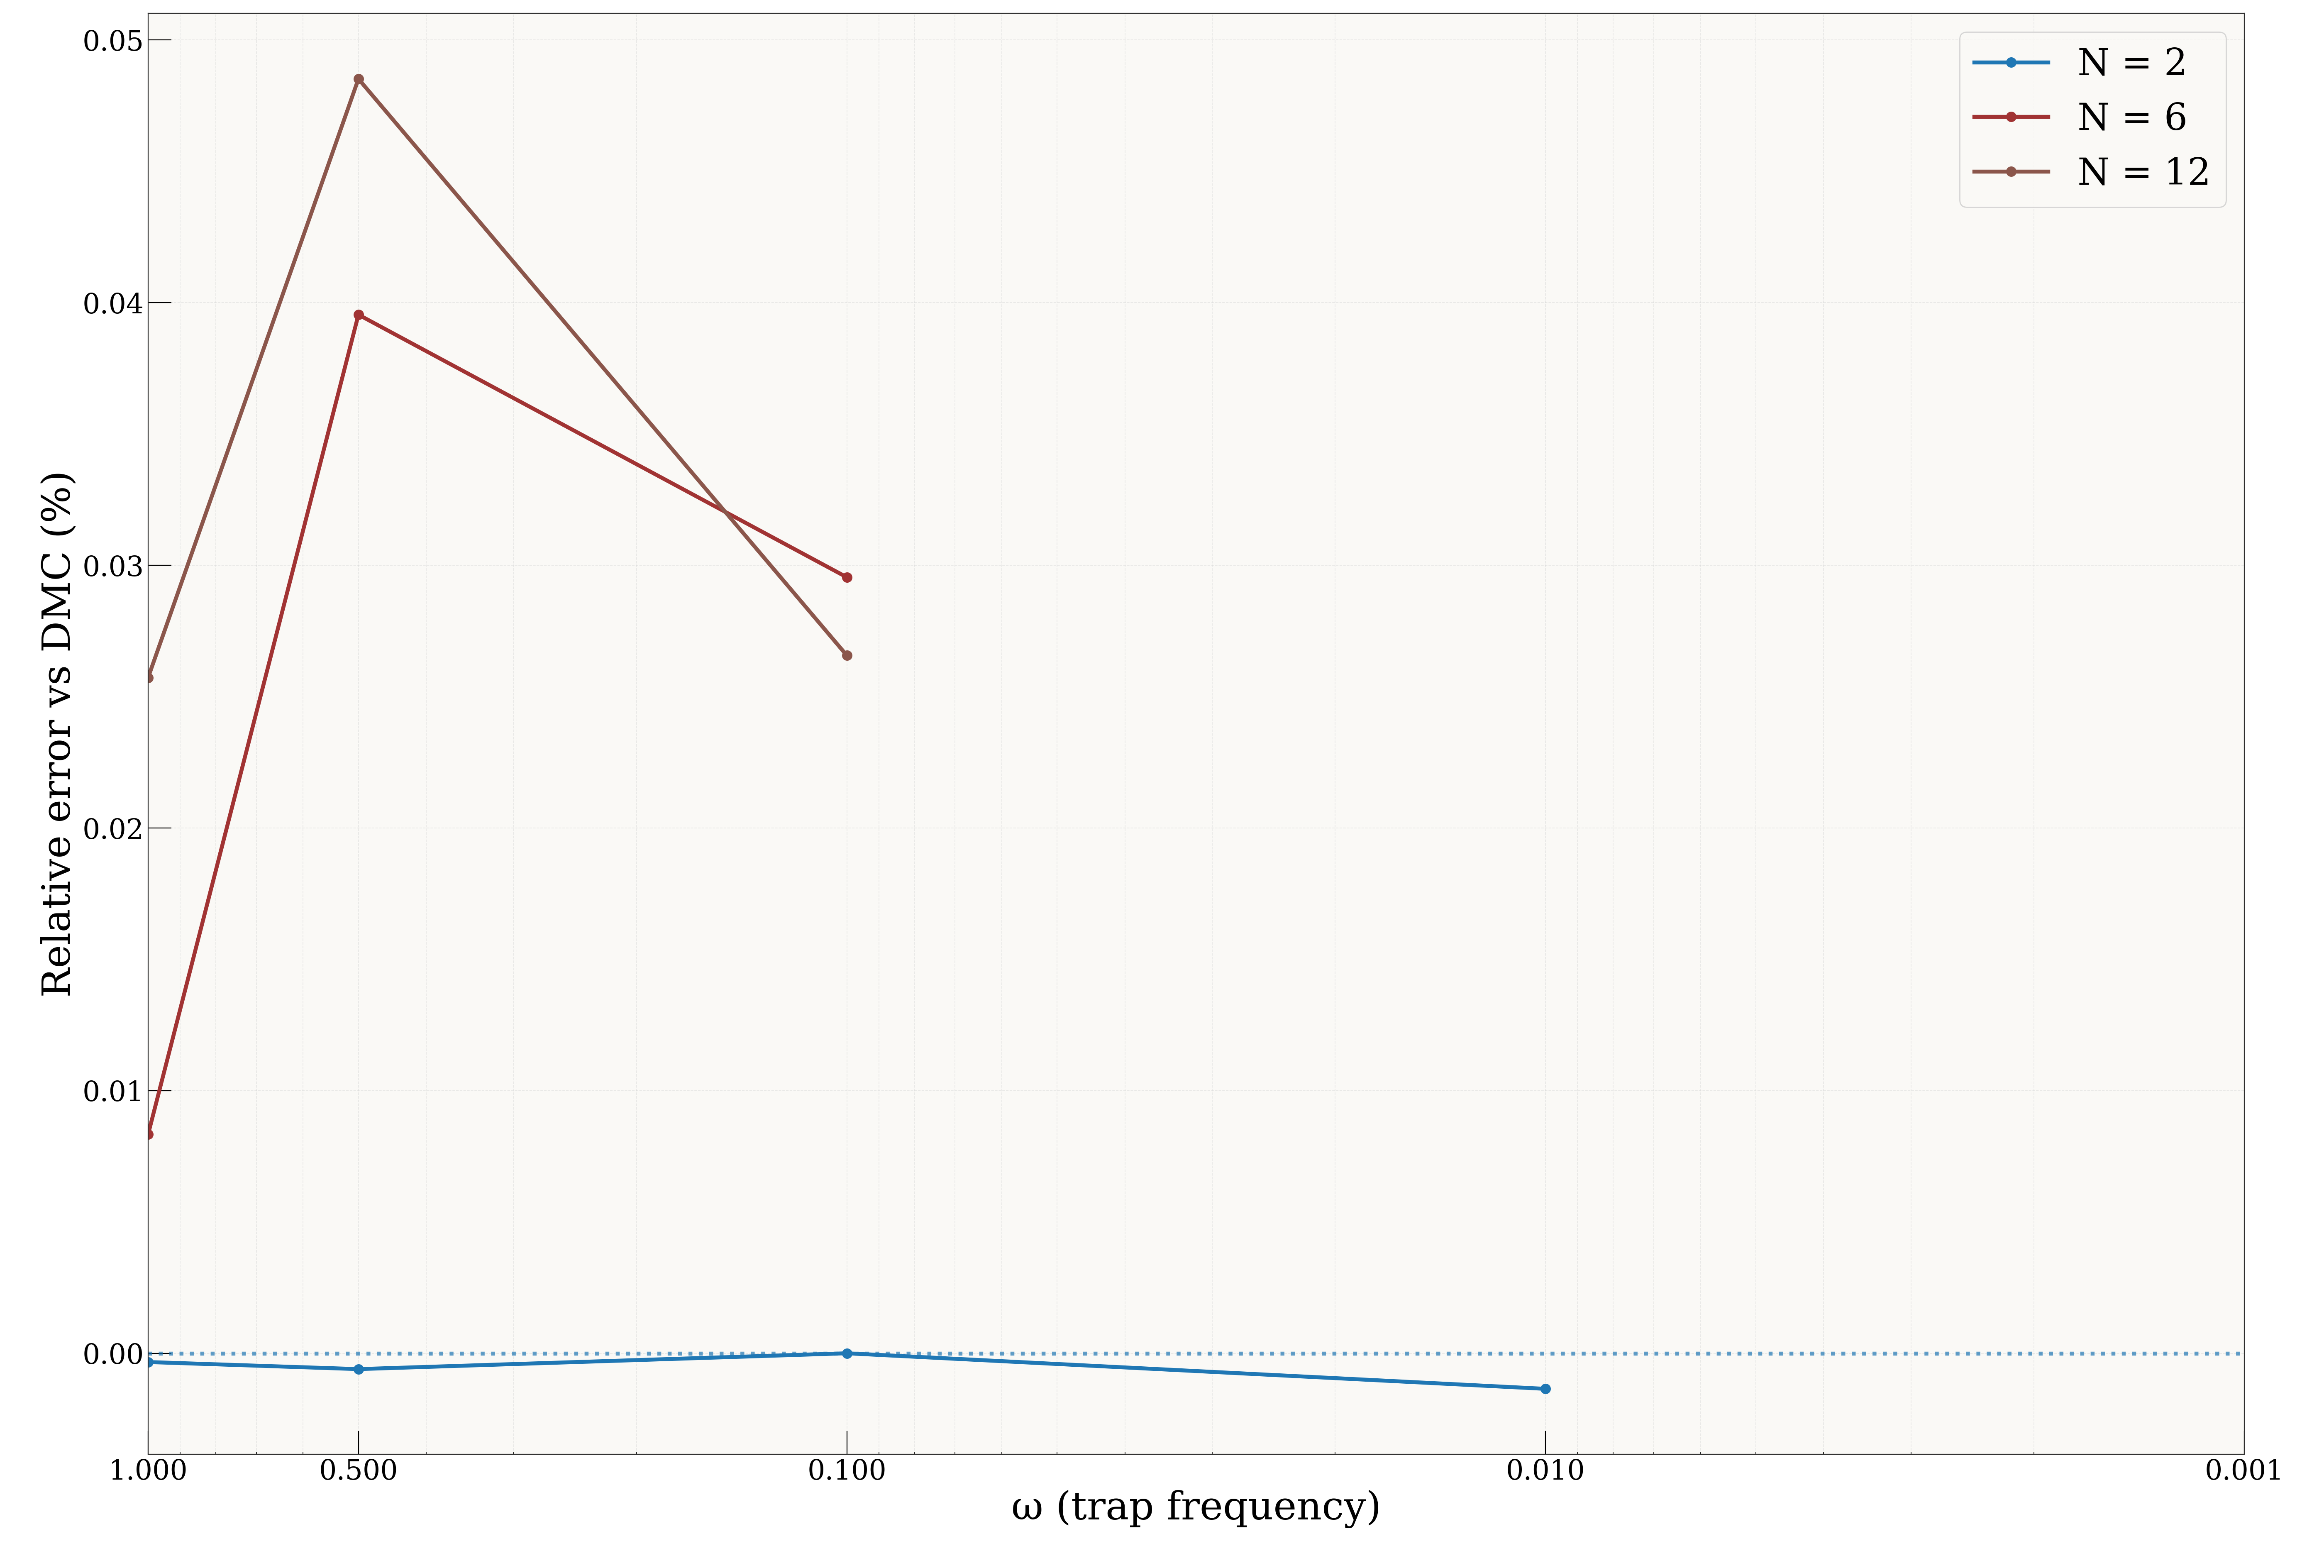
\includegraphics[width=0.9\textwidth]{rel_error_vs_omega_allN}
  \caption[Relative deviation from the external references]{Relative deviation of the conv.-BF
  energies from the external references (Table~\ref{tab:energies}) at every $(N,\omega)$
  where one exists: fixed-node DMC~\cite{Hogberget2013-DMC} for $N{=}6$ and $12$, and the
  compiled DMC and analytic~\cite{Taut1994-TwoElectrons} values for $N{=}2$. Deviations are at
  the $10^{-3}\,\%$ level for $N{=}2$, comparable to the reference's own precision, and
  $0.008$--$0.05\,\%$ for $N{=}6$ and $12$, with no trend in $\omega$.}
  \label{fig:rel_error_vs_omega}
\end{figure}

\FloatBarrier
\paragraph{The same benchmark, without a Markov chain.}
Everything above was trained with a Markov chain: residual pretraining, then an SR tail
that draws its samples from $|\Psi|^2$ by Metropolis. A second route removes the chain from
the gradient entirely, replacing it with an analytic proposal and importance weights. It
reaches comparable energies over part of this range. Its performance, its failure boundary
and the mechanism behind both are the subject of \S\ref{sec:kernel-mcmcfree}, and the
energies are tabulated there (Table~\ref{tab:collocation}) and not here, because they
are not interpretable until that mechanism is in hand.

\paragraph{Where the tables stop.}
One subtlety matters here, because the MP-BF ansatz sits \emph{below} the quoted DMC
reference in four cells, and at $N{=}12$ and $N{=}20$, $\omega=1$, by more than ten combined
standard errors (for example $65.6956$ vs.\ $65.7001$\,Ha at $N{=}12$). This does not violate
the variational principle, which bounds the energy from below only by the \emph{exact}
ground state, $E_{\rm VMC}\ge E_0$; the DMC benchmarks are \emph{fixed-node} calculations
and carry their own nodal bias. A better nodal surface in the network would produce exactly
this pattern. It is not the only thing that would, but one alternative can be set aside. A
difference in the convention for the Hamiltonian or its units is ruled out: the same ansatz
reproduces the exact two-electron value $3.00000$ at $\omega=1$, and a convention mismatch
would shift every cell, not four. What remains is a time-step or population extrapolation in
the reference, an underestimated statistical error on either side, or an error somewhere in
the chain of compilations by which the reference reached us (see the notes to
Table~\ref{tab:energies}), and nothing here distinguishes these from better nodes. The clean test is a fixed-node DMC
calculation that uses the network's own nodes as its trial surface, which we have not run.
The sub-reference values are therefore recorded as deviations and not interpreted.

Wherever an external check exists, the pattern is the same. For $N{=}2$ the ansatz reaches reference
accuracy at every $\omega$ at which it is compared with one, and for $N\!\in\!\{6,12\}$
the relative deviation stays within $0.008$–$0.05\%$ across the benchmarked
range ($\omega\ge0.1$; Fig.~\ref{fig:rel_error_vs_omega}). Below $\omega=0.1$ there
is no DMC reference for $N\ge6$, and we make no claim of absolute accuracy there;
what we can say is that the energies join smoothly onto the benchmarked regime and, in
the deep-Wigner limit, follow a power law whose fitted exponent, $0.689$ for $N{=}6$
(\S\ref{sec:kernel-q3-frontier}), sits close to the classical Wigner value $2/3$. The efficiency is as notable as the accuracy: the SR
tail converges in $10^3$–$3\times10^3$ iterations of $\sim 3{\times}10^3$ samples
each, a modest optimisation budget for a fully many-body wavefunction. We attribute
this stability to a small set of conditioning choices---
trap-unit scaling, soft-core pair features with $ds/dr\!\to\!0$ at coalescence, and
an explicit analytic cusp---each of which keeps the gradients and the Laplacian
numerically tame from the shallowest trap to the tightest.

\section{Wigner--molecule crossover}
\label{sec:wigner-molecule}

Up to this point the wavefunction has been the thing under examination. Here it becomes
the instrument.

\textbf{The result of this section is that the crossover is staged.} As the trap weakens the
cloud first expands and its shells stiffen \emph{radially}---the width-to-radius ratio
falls, discrete occupancies emerge, the energy partition approaches classical force
balance---while the electrons remain very nearly disordered in angle within those shells.
Angular structure then develops in two steps of its own: a small, gradually growing
correlation that is measurable well before the Wigner regime, and a large
bond-orientational ordering confined to the final decade of confinement. Against the
random-angle baseline the shell bond order runs at $0.99$--$1.01$ of its null value from
$\omega=1$ down to $\omega=0.1$, reaches $1.08$ at $\omega=0.01$ for $N{=}6$ (and stays
within $1.02$ at $N{=}12$ and $N{=}20$), and only at $\omega=10^{-3}$ jumps to $1.16$--$1.63$
on every ring at every particle number. Radial localisation and angular crystallisation are
not one transition, and the diagnostics below are arranged to separate them.

\paragraph{Which states these are.}
Every state in this section is the lowest we find with $N_\uparrow=N_\downarrow$ held fixed,
starting from the closed-shell singlet of the non-interacting problem. That is not a
formality here. Fixing the spin projection does not fix the total spin, since an $S=1$ state
also has an $S_z=0$ component, and we never compare sectors of different $S$. In parabolic
dots the interaction is known to drive spin transitions as it strengthens---for instance
$S=0\!\to\!S=1$ at $N=6$ in the strongly correlated regime~\cite{Egger_1999}---so a change
of ground-state spin is plausible precisely at the weakest traps, where the structural
conclusions below are strongest. The deep-Wigner states are therefore the lowest states
found within a fixed spin-projection sector, not established global ground states, and
every statement below is about them. There is a reason to expect the \emph{charge}
geometry to be less sensitive than the energy ordering---deep in the Wigner regime exchange
is weak and states of different $S$ become nearly degenerate over the same classical
arrangement---but that is an expectation we have not tested, not a result.

The subsections take that in order. \S\ref{sec:wigner-onebody} shows the cloud expanding and
acquiring visible radial structure; \S\ref{sec:wigner-energy} shows interactions taking over
and the trap--interaction partition approaching its classical form;
\S\ref{sec:wigner-radial} shows the shells stiffening radially; and
\S\ref{sec:wigner-angular} shows angular order finally appearing, tested against a null in
which the angles are random. \S\ref{sec:wigner-synthesis} collects what the diagnostics
agree on and what they do not establish.

What we are looking for cannot be seen in the observable one would naturally plot. In a
rotationally symmetric trap, the electrons of a Wigner molecule localise in \emph{relative} coordinates (concentric rings, polygon-like angular correlations) while the whole pattern is free to rotate. Average over that rotation, as
any lab-frame density does, and the rings smear into something close to uniform. The
order is there; the density hides it. Every diagnostic below exists to look past that
averaging.

We combine one-body densities, label-invariant shell topology, rotation-registered
angular order, shell radii and gaps, pair statistics, and Lindemann-type disorder, across
$N=2,6,12,20$ and $\omega\in\{1,0.5,0.1,0.01,0.001\}$~\cite{Egger_1999,manninen2007metalclustersquantumdots}.
No one of them is decisive on its own. They fail in different ways, which is why they are
reported together.

% ──────────────────────────────────────────────────────────────────────
\subsection{Observables and diagnostics}
\label{sec:wigner-diagnostics}

For each $(N,\omega)$ we draw $\mathbf X\!\sim|\Psi|^2$ and report
(i)~the pair distribution $g(r)$,
(ii)~the single-particle radial density $P(r)\!\propto\!r\,\rho(r)$,
and summary statistics: $r_{\rm mode}$, $\langle r\rangle$, $\sigma_r$, FWHM,
quantiles $q_{10},q_{50},q_{90}$, and a localisation ratio
$\gamma=\sigma_r/r_{\rm mode}$ (smaller $\gamma$ $\Rightarrow$ stiffer
localisation).
For multi-electron systems we additionally monitor shell-resolved
bond-orientational order $|\Phi_m|$ and a dimensionless Lindemann-type
ratio for positional fluctuations on each
ring~\cite{Mazars_2008}.

\paragraph{Density parameter $r_s$.}
Following Egger \textit{et al.}~\cite{Egger_1999}, we estimate the Wigner--Seitz
parameter from the first maximum $r^\ast$ of the spin-summed pair correlation,
$r_s\equiv r^\ast/a_B^\ast$.
The Fermi--liquid $\to$ Wigner--molecule crossover occurs near $r_s\!\simeq\!4$
in parabolic dots; our weak-trap cases lie well beyond this
threshold~\cite{Egger_1999,Filinov_2001}.

% ──────────────────────────────────────────────────────────────────────
\subsection{One-body densities: visual crossover}
\label{sec:wigner-onebody}

Figures~\ref{fig:onebody_grid} and~\ref{fig:onebody_n20} compare one-body
densities at strong confinement ($\omega=1$) and weak confinement
($\omega=10^{-3}$) for $N=2,6,12,20$.
At $\omega=1$ the density remains compact and the dominant change with $N$ is
progressive shell filling under the harmonic trap. At $\omega=10^{-3}$ it broadens by two
orders of magnitude and develops pronounced \emph{radial} structure at every $N$.

What that structure can and cannot establish follows from the symmetry argument above. The
lab-frame density is an average over all orientations of the molecule, so it retains radial
information and destroys angular information by construction. These figures are therefore
evidence of \emph{radial shell localisation} and are silent on whether the electrons are
angularly ordered within those shells---a ring of six electrons at fixed $60^\circ$ spacing
and six electrons sliding freely around the same ring produce the same picture. The angular
question is taken up in \S\ref{sec:wigner-angular}, where it needs a co-rotating frame and a
null model to answer.

\begin{figure*}[htbp]
  \centering
  \captionsetup[subfigure]{justification=centering,font=small}

  % ---------- Row 1: ω = 1.0 ----------
  \begin{subfigure}[t]{\threecolw}
    \centering
    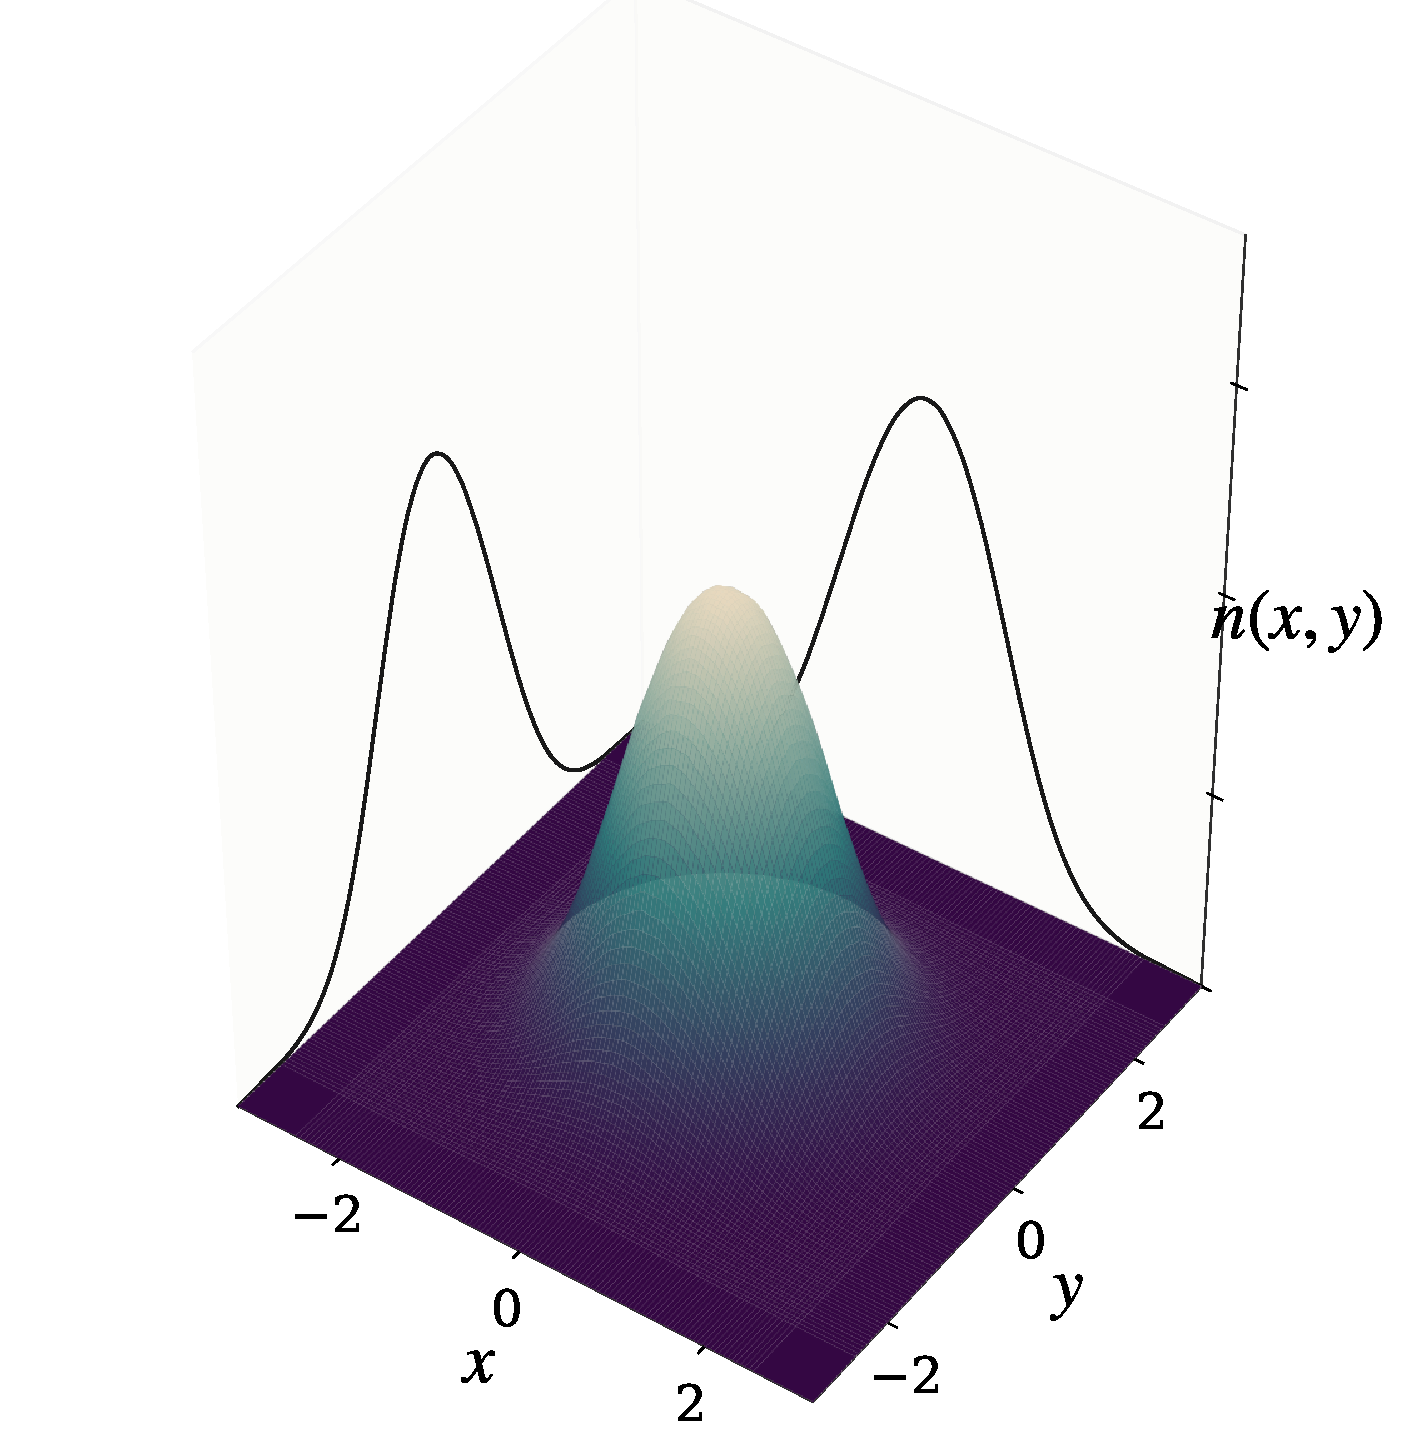
\includegraphics[width=\linewidth]{one_body_density_2_omega_1.00000_20251029_231309.pdf}
    \caption{$N{=}2,\;\omega=1.0$}
  \end{subfigure}\hspace{\figgutter}%
  \begin{subfigure}[t]{\threecolw}
    \centering
    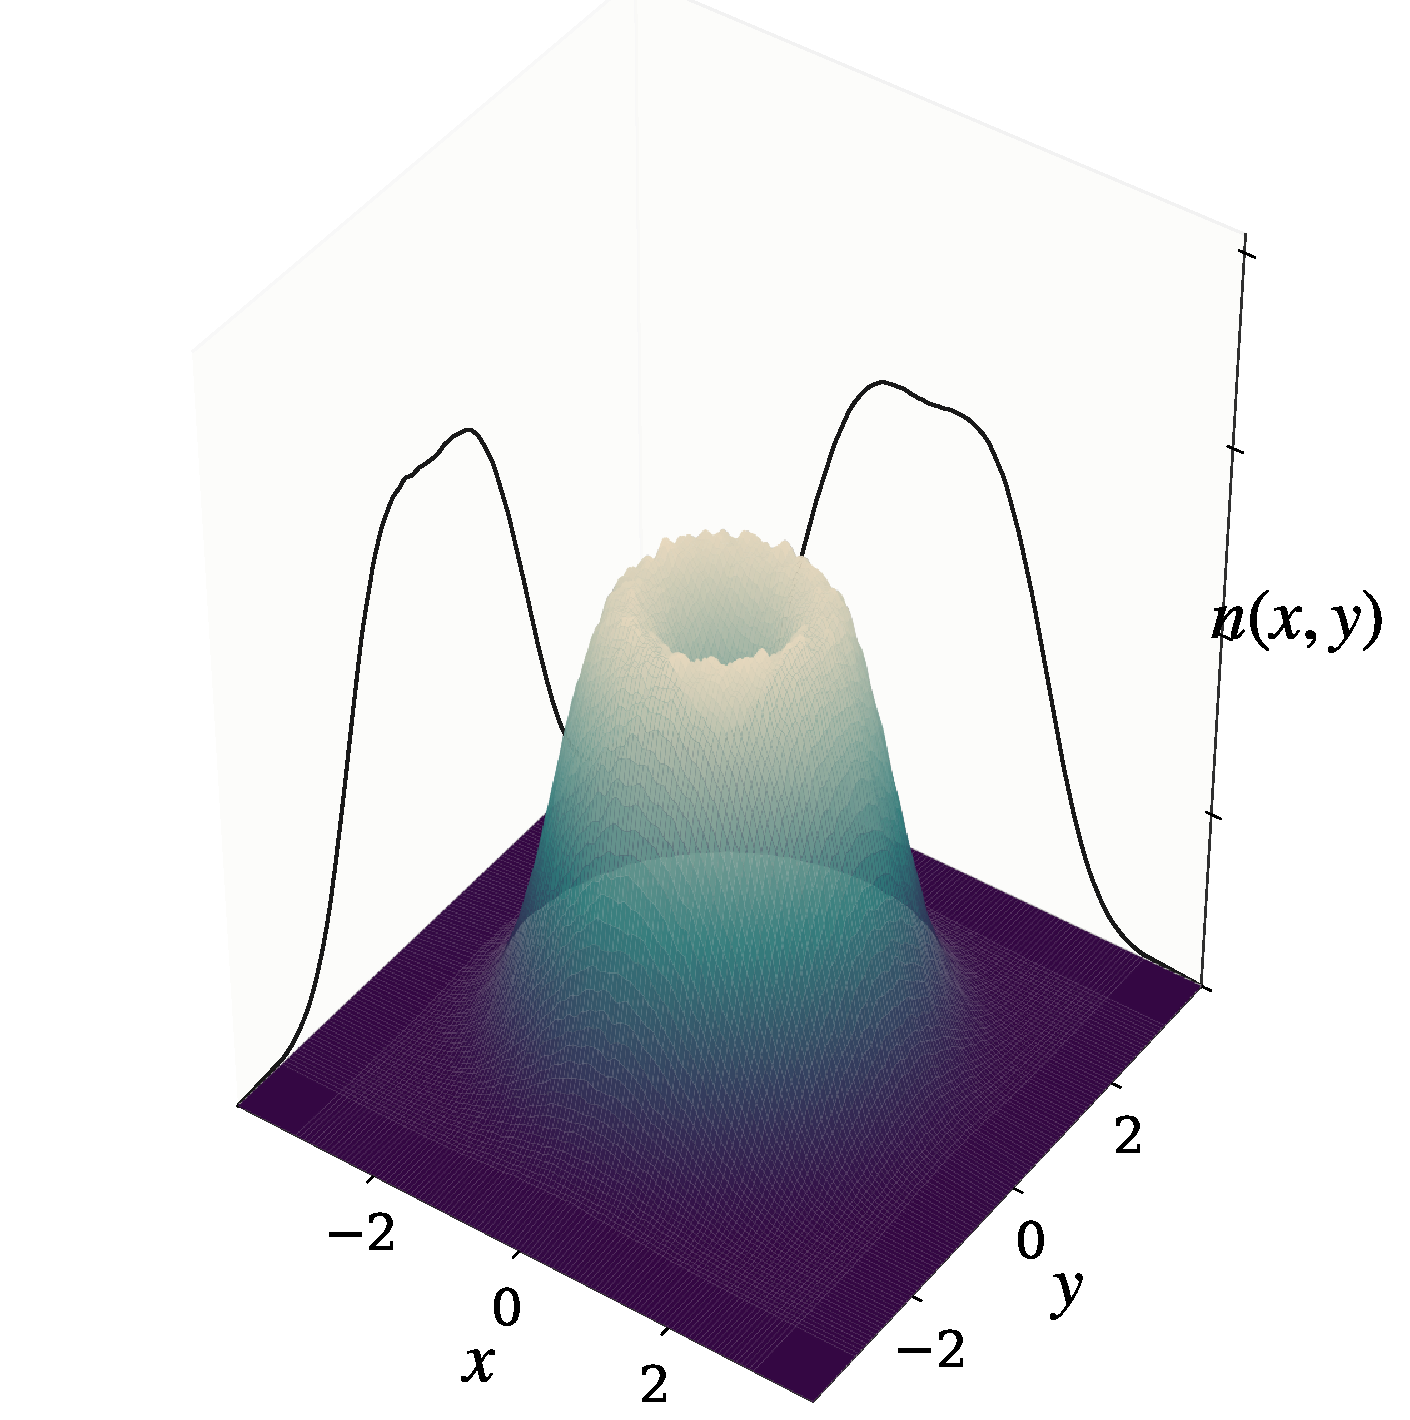
\includegraphics[width=\linewidth]{one_body_density_6_omega_1.00000_20251030_093439.pdf}
    \caption{$N{=}6,\;\omega=1.0$}
  \end{subfigure}\hspace{\figgutter}%
  \begin{subfigure}[t]{\threecolw}
    \centering
    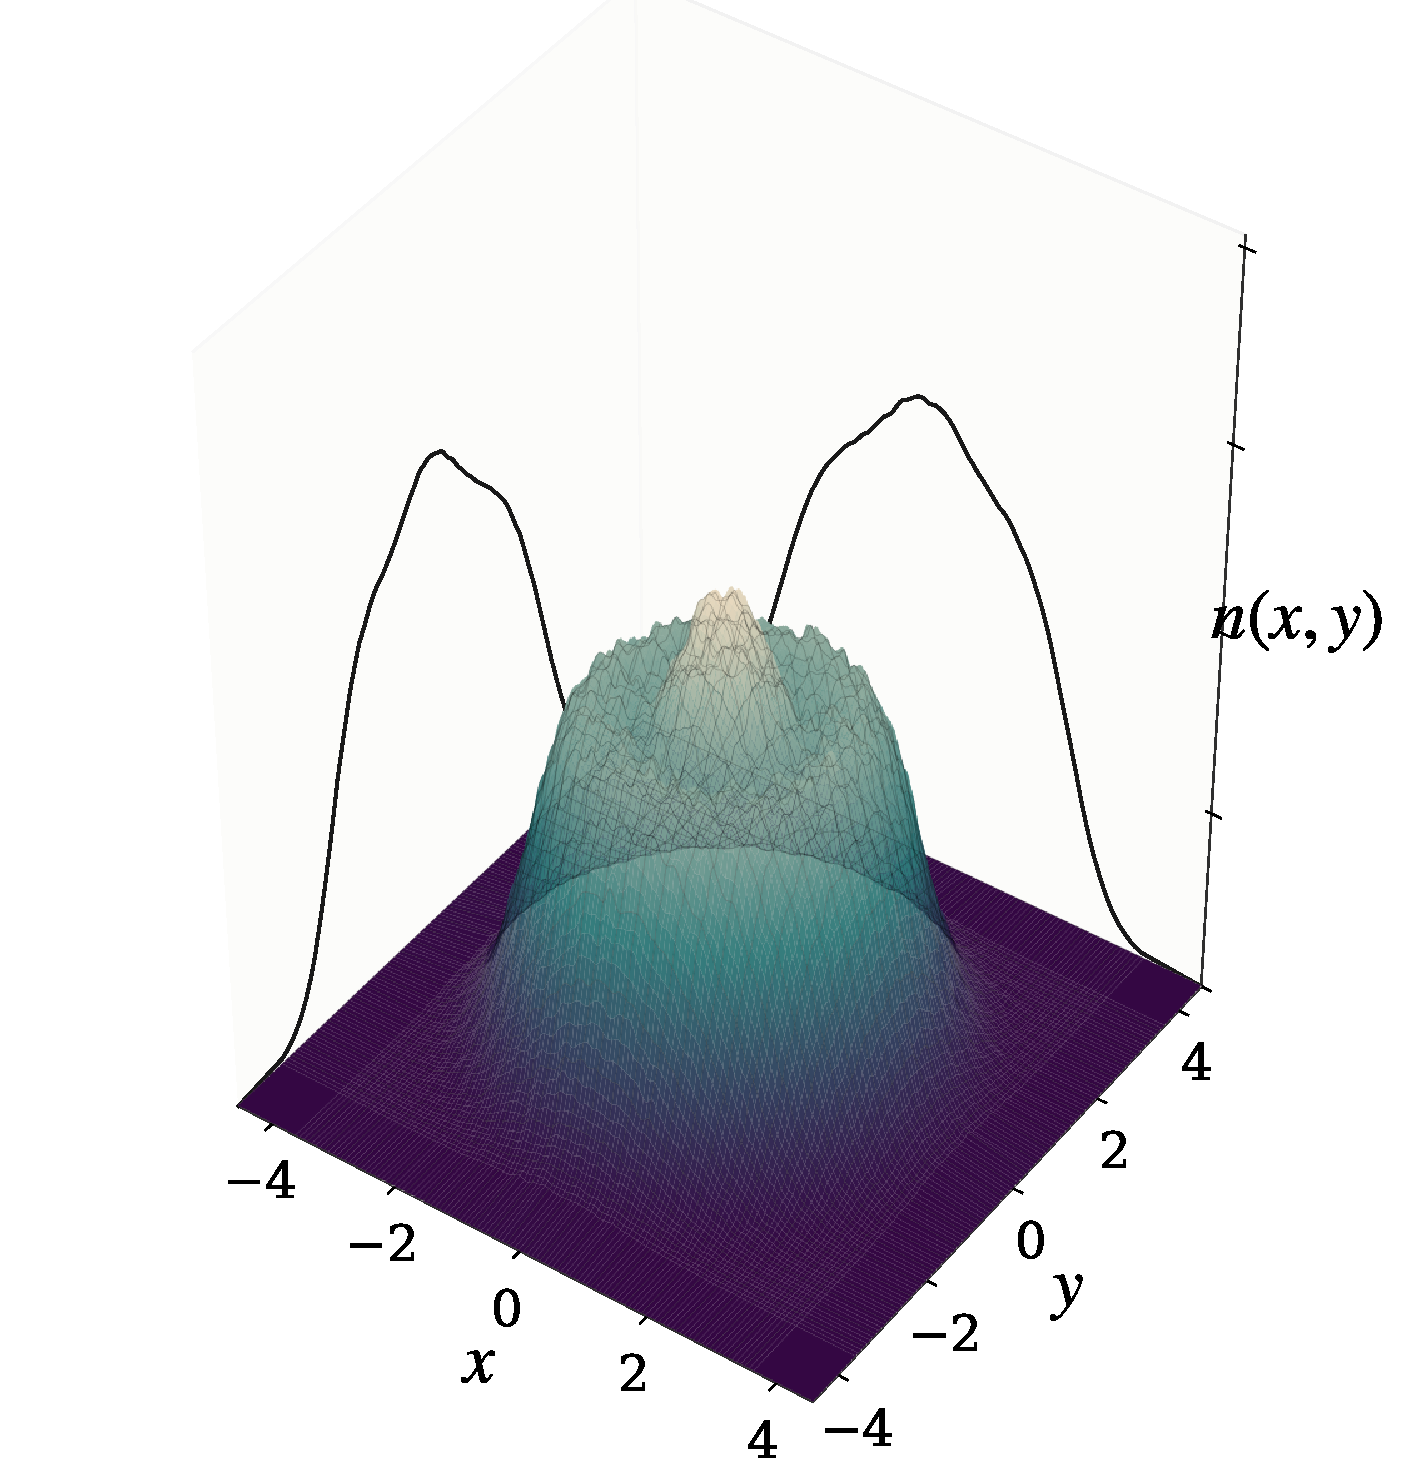
\includegraphics[width=\linewidth]{one_body_density_12_omega_1.00000_20251104_194000.pdf}
    \caption{$N{=}12,\;\omega=1.0$}
  \end{subfigure}

  \vspace{0.5em}

  % ---------- Row 2: ω = 0.001 ----------
  \begin{subfigure}[t]{\threecolw}
    \centering
    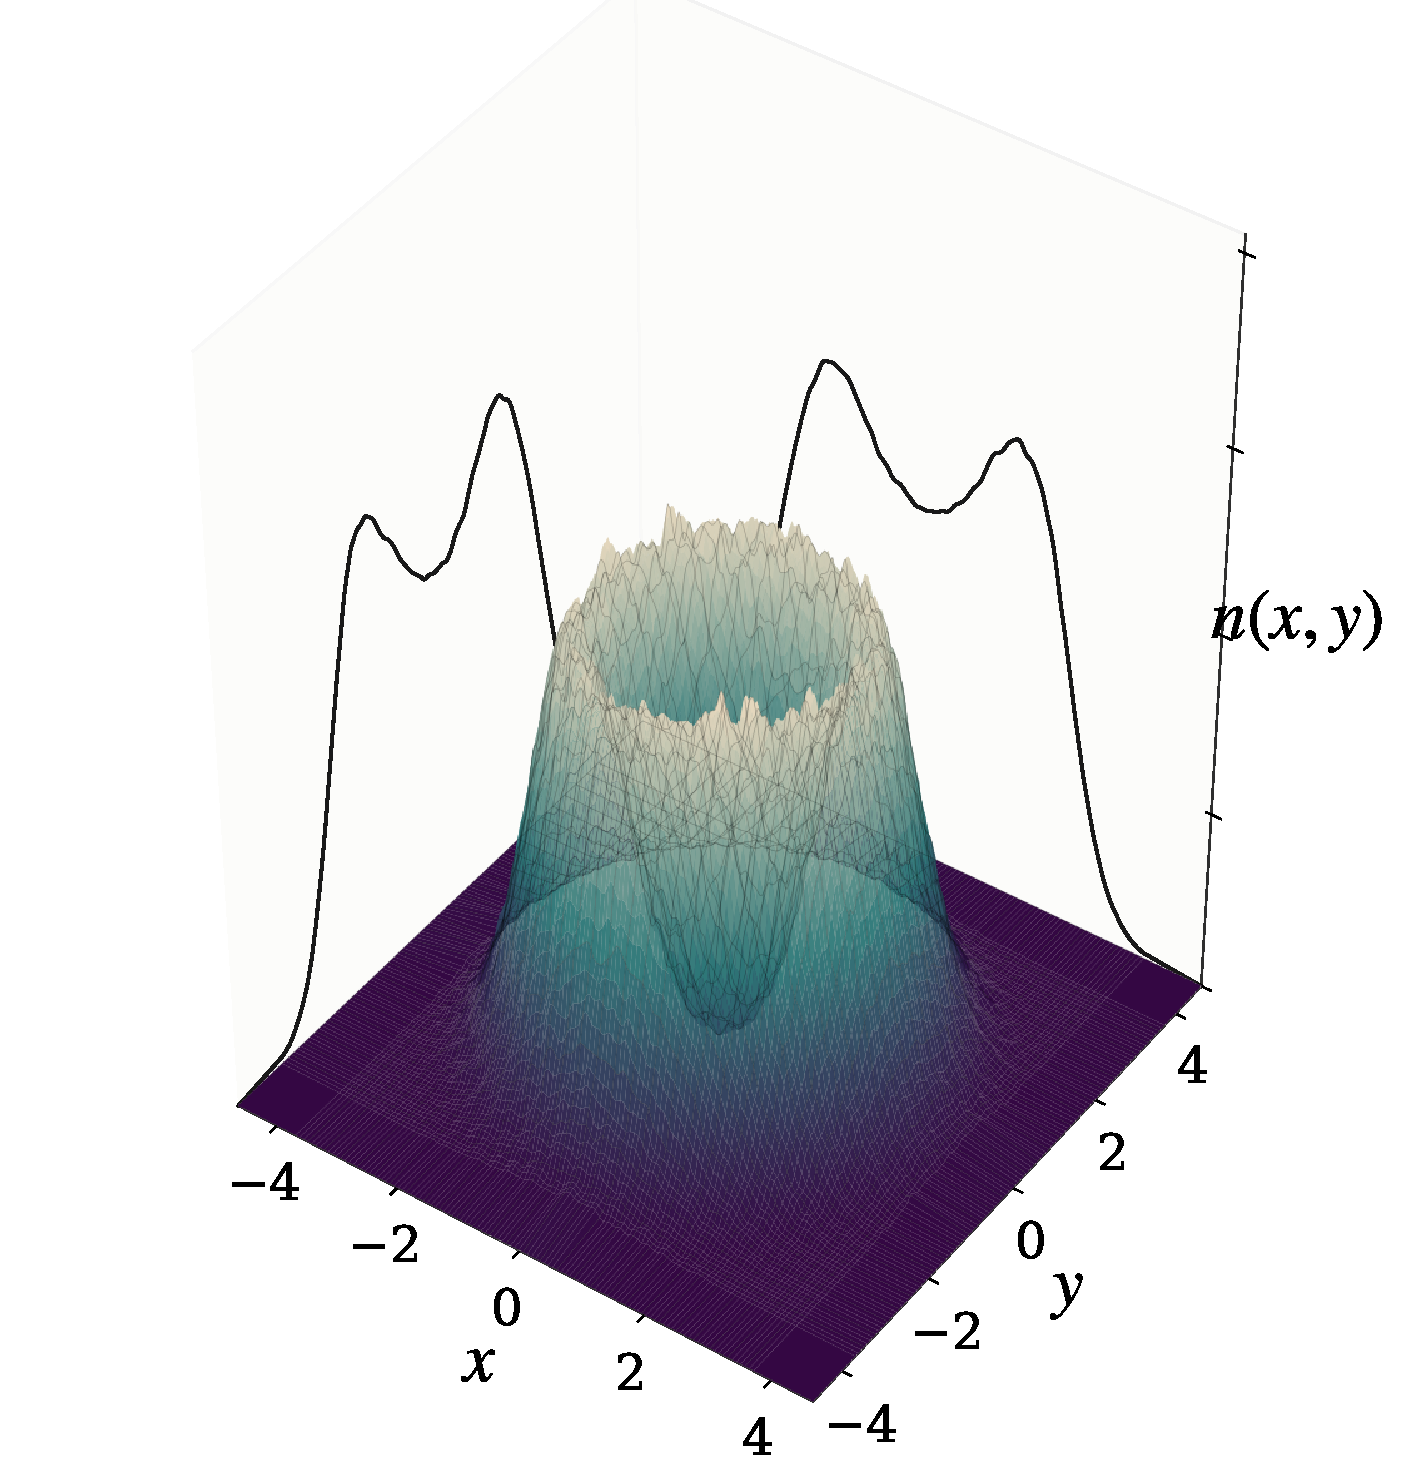
\includegraphics[width=\linewidth]{one_body_density_2_omega_0.00100_20251106_160757.pdf}
    \caption{$N{=}2,\;\omega=0.001$}
  \end{subfigure}\hspace{\figgutter}%
  \begin{subfigure}[t]{\threecolw}
    \centering
    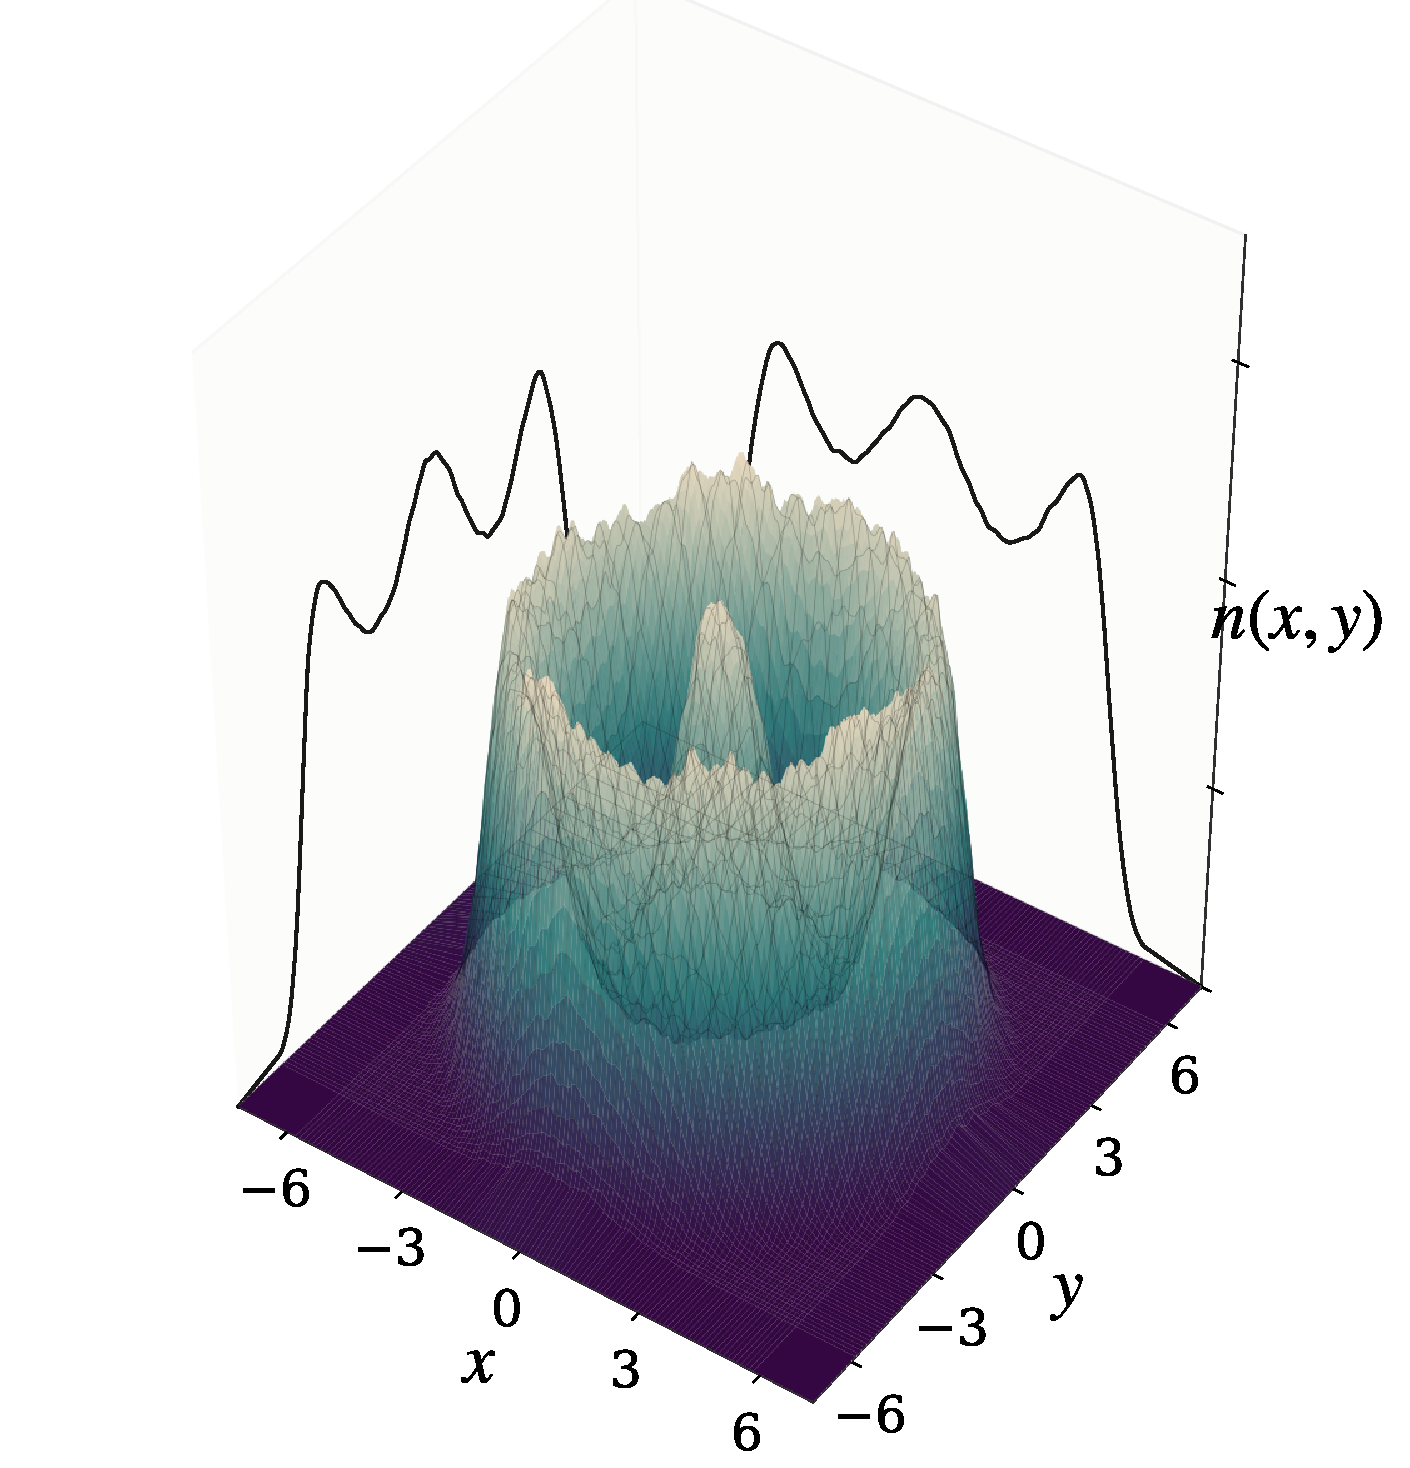
\includegraphics[width=\linewidth]{one_body_density_6_omega_0.00100_20251106_214930.pdf}
    \caption{$N{=}6,\;\omega=0.001$}
  \end{subfigure}\hspace{\figgutter}%
  \begin{subfigure}[t]{\threecolw}
    \centering
    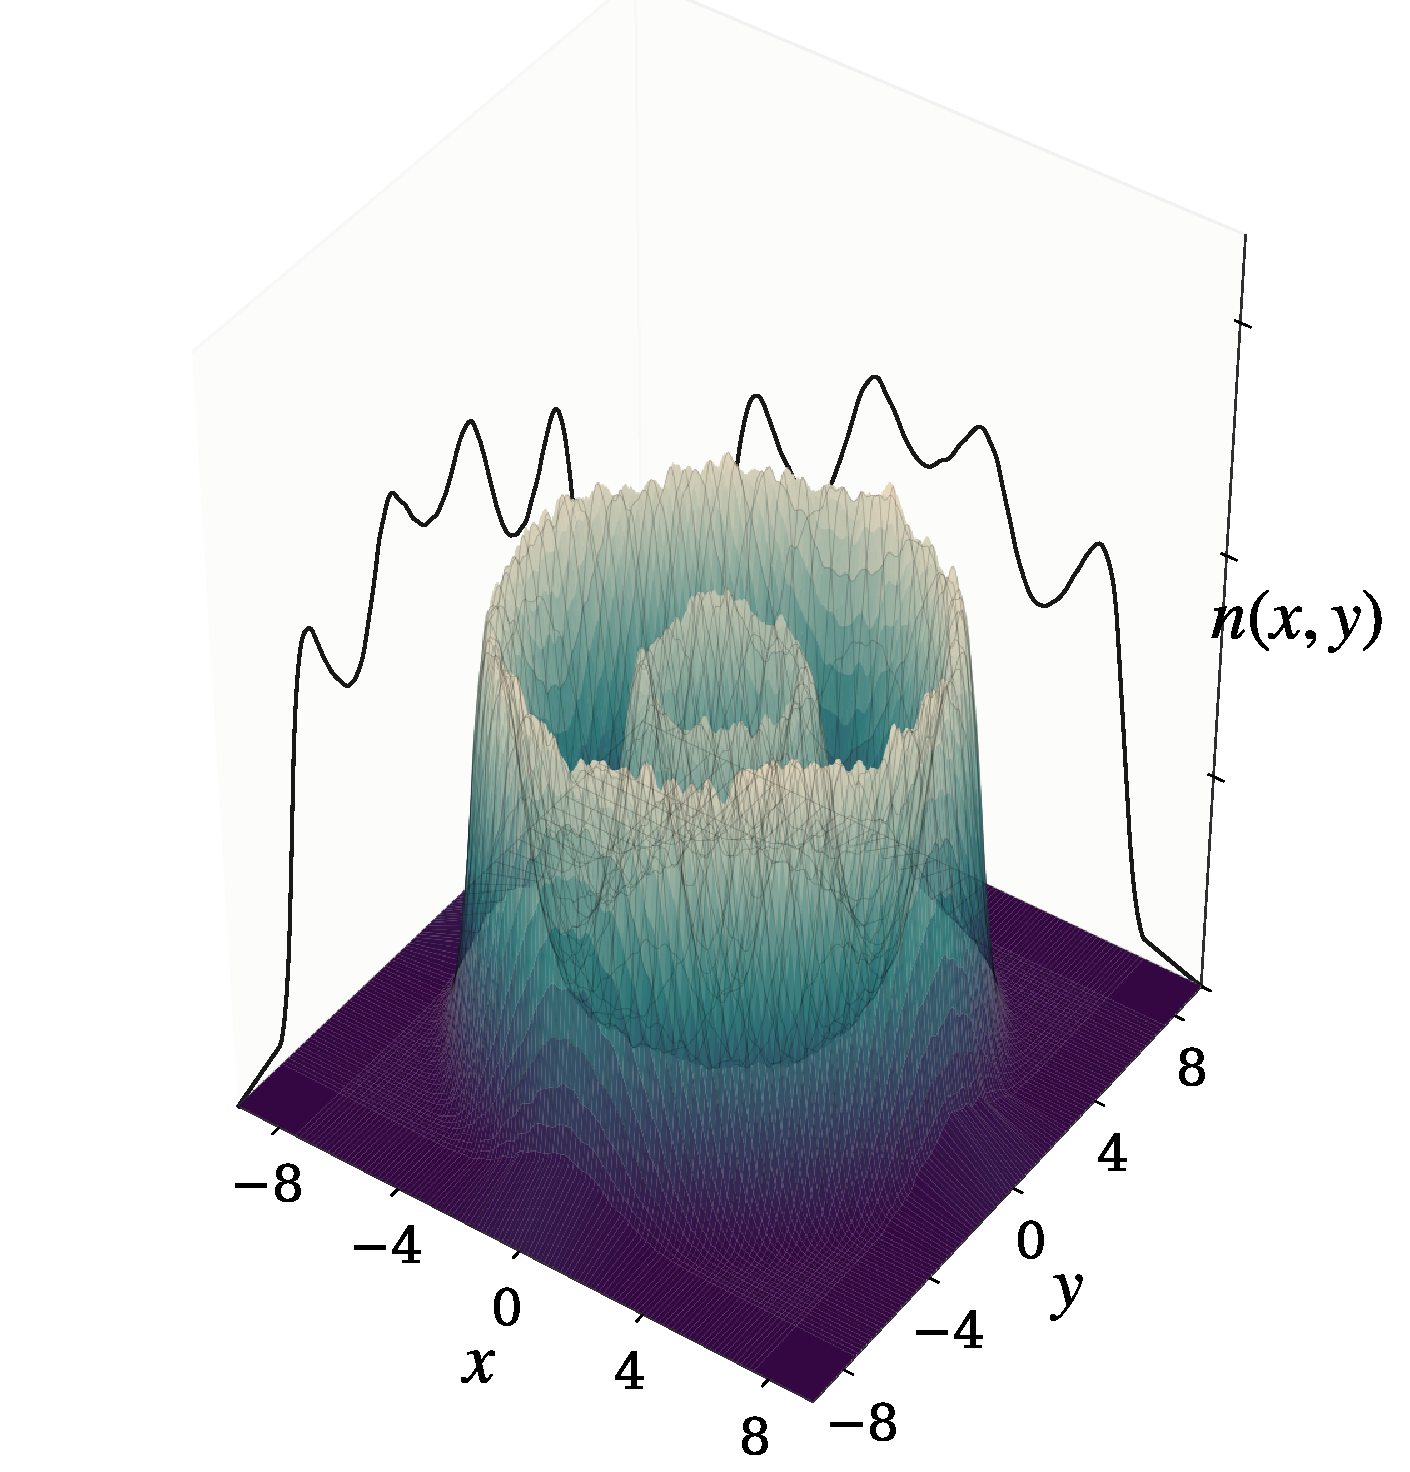
\includegraphics[width=\linewidth]{one_body_density_12_omega_0.00100_20251109_110913.pdf}
    \caption{$N{=}12,\;\omega=0.001$}
  \end{subfigure}

  \caption[One-body densities at strong and weak confinement, $N=2,6,12$]{One-body
  densities for $N=2,6,12$ at $\omega=1.0$ (top) and $\omega=0.001$ (bottom). The vertical
  axis is the one-body density $n(x,y)$ over the two Cartesian components of a single
  particle's position, in trap units; the curves on the back walls are its marginals. As
  confinement weakens the densities broaden
  and develop pronounced \emph{radial} shell structure. Being lab-frame averages over all
  orientations of the molecule, they cannot show angular order: that requires the registered
  diagnostics of \S\ref{sec:wigner-angular}.}
  \label{fig:onebody_grid}
\end{figure*}

\begin{figure}[htbp]
  \centering
  \captionsetup[subfigure]{justification=centering,font=small}
  \begin{subfigure}[t]{0.48\textwidth}
    \centering
    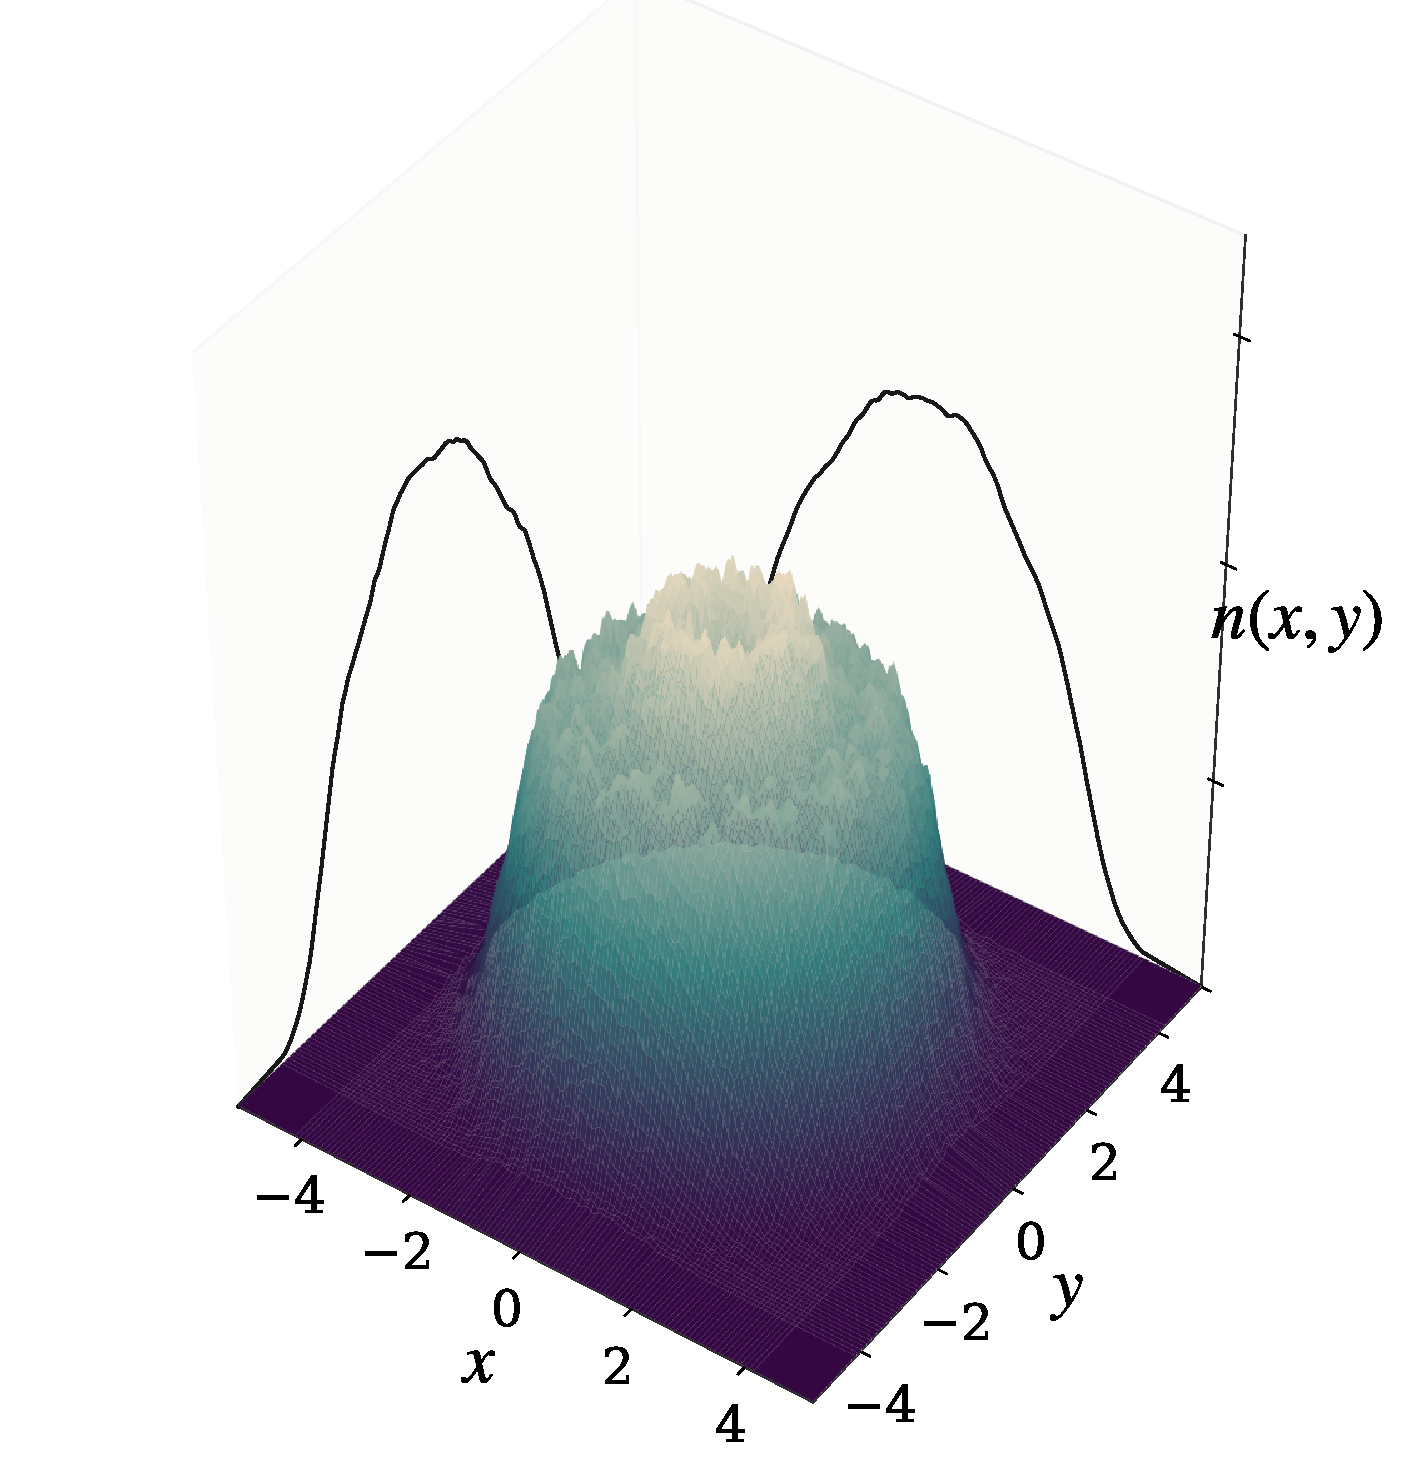
\includegraphics[width=\linewidth]{one_body_density_20_omega_1.00000_20251228_180301.pdf}
    \caption{$N{=}20,\;\omega=1.0$}
  \end{subfigure}
  \hfill
  \begin{subfigure}[t]{0.48\textwidth}
    \centering
    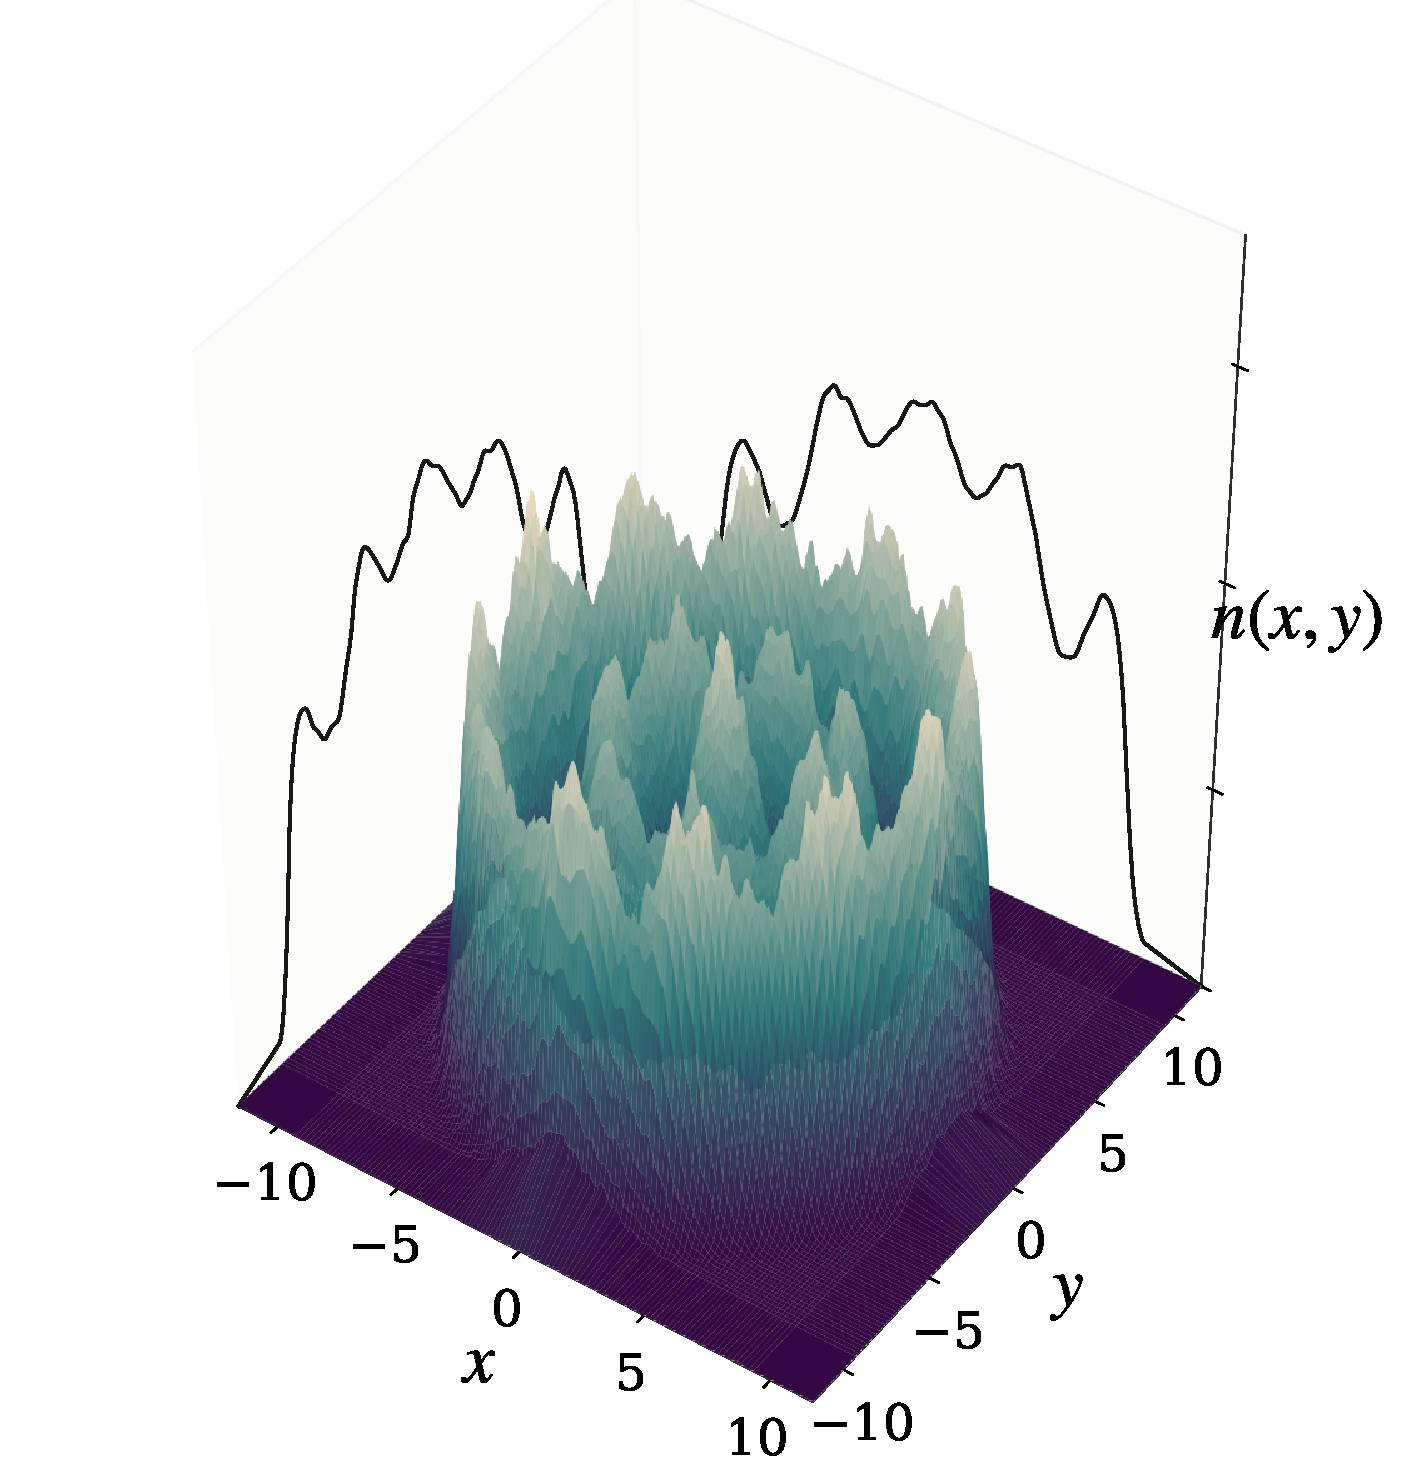
\includegraphics[width=\linewidth]{one_body_density_20_omega_0.00100.pdf}
    \caption{$N{=}20,\;\omega=0.001$}
  \end{subfigure}
  \caption[One-body densities at strong and weak confinement, $N{=}20$]{One-body densities
  for $N{=}20$ at strong and weak confinement; the vertical axis is $n(x,y)$ as in
  Fig.~\ref{fig:onebody_grid}. The weak-trap case shows strong radial broadening and clear
  multi-shell organisation. As above, this is radial evidence only.}
  \label{fig:onebody_n20}
\end{figure}

% ──────────────────────────────────────────────────────────────────────
\subsection{Energy-based crossover diagnostics}
\label{sec:wigner-energy}

\begin{figure*}[htbp]
  \centering
  \captionsetup[subfigure]{justification=centering}

  \begin{subfigure}[t]{0.48\textwidth}
    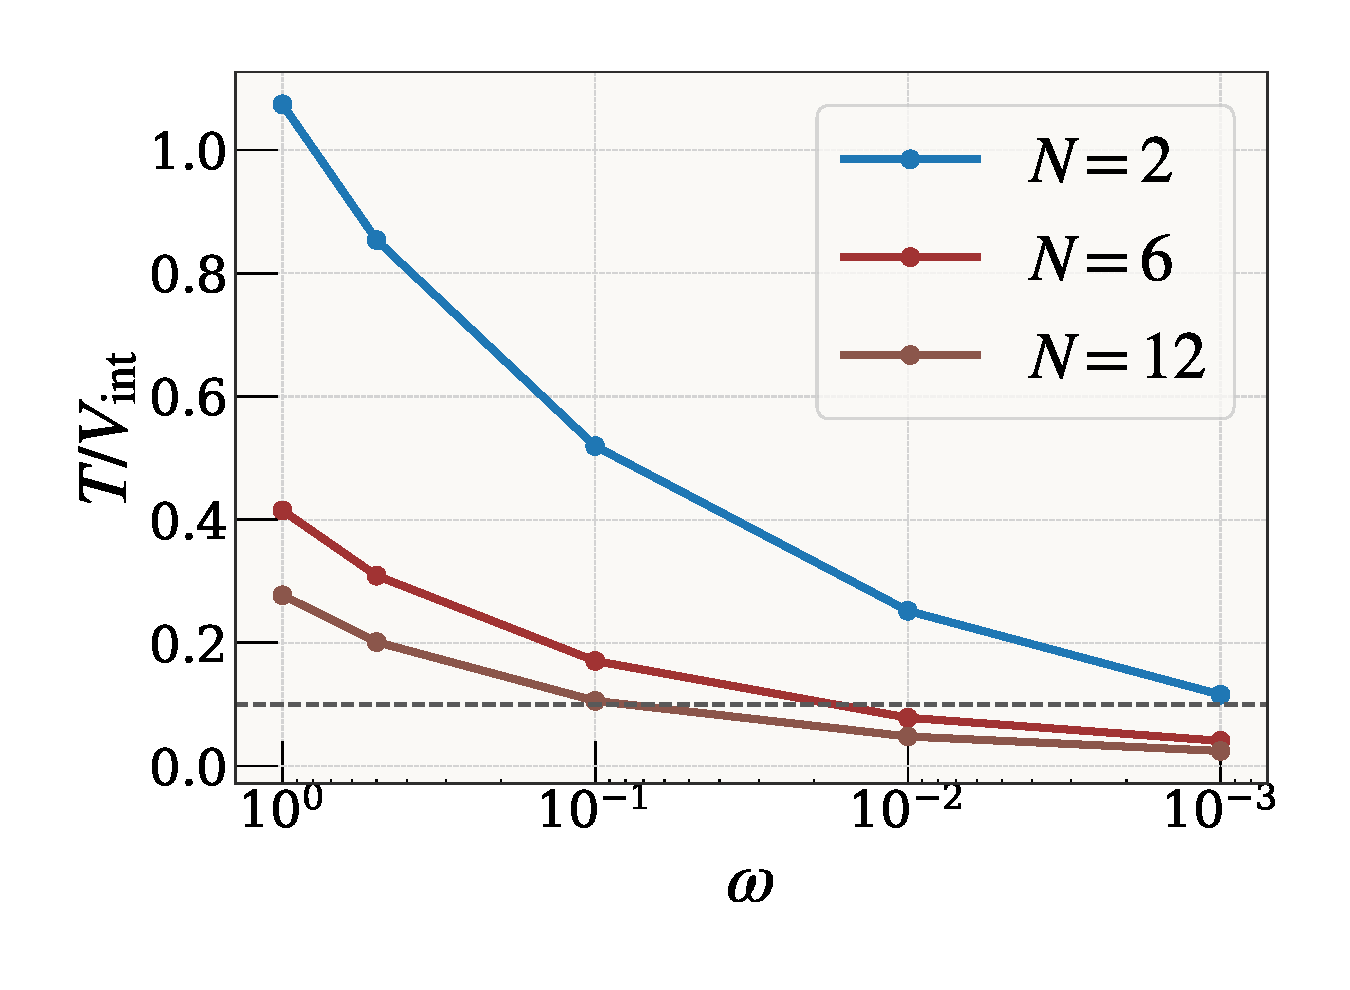
\includegraphics[width=\linewidth]{ratio_T_over_Vint_desc_allN}
    \caption[]{$T/V_{\rm int}$ vs.\ $\omega$ for $N{=}2,6,12$.
    The horizontal line marks $T/V_{\rm int}{=}0.1$.}
  \end{subfigure}
  \hfill
  \begin{subfigure}[t]{0.48\textwidth}
    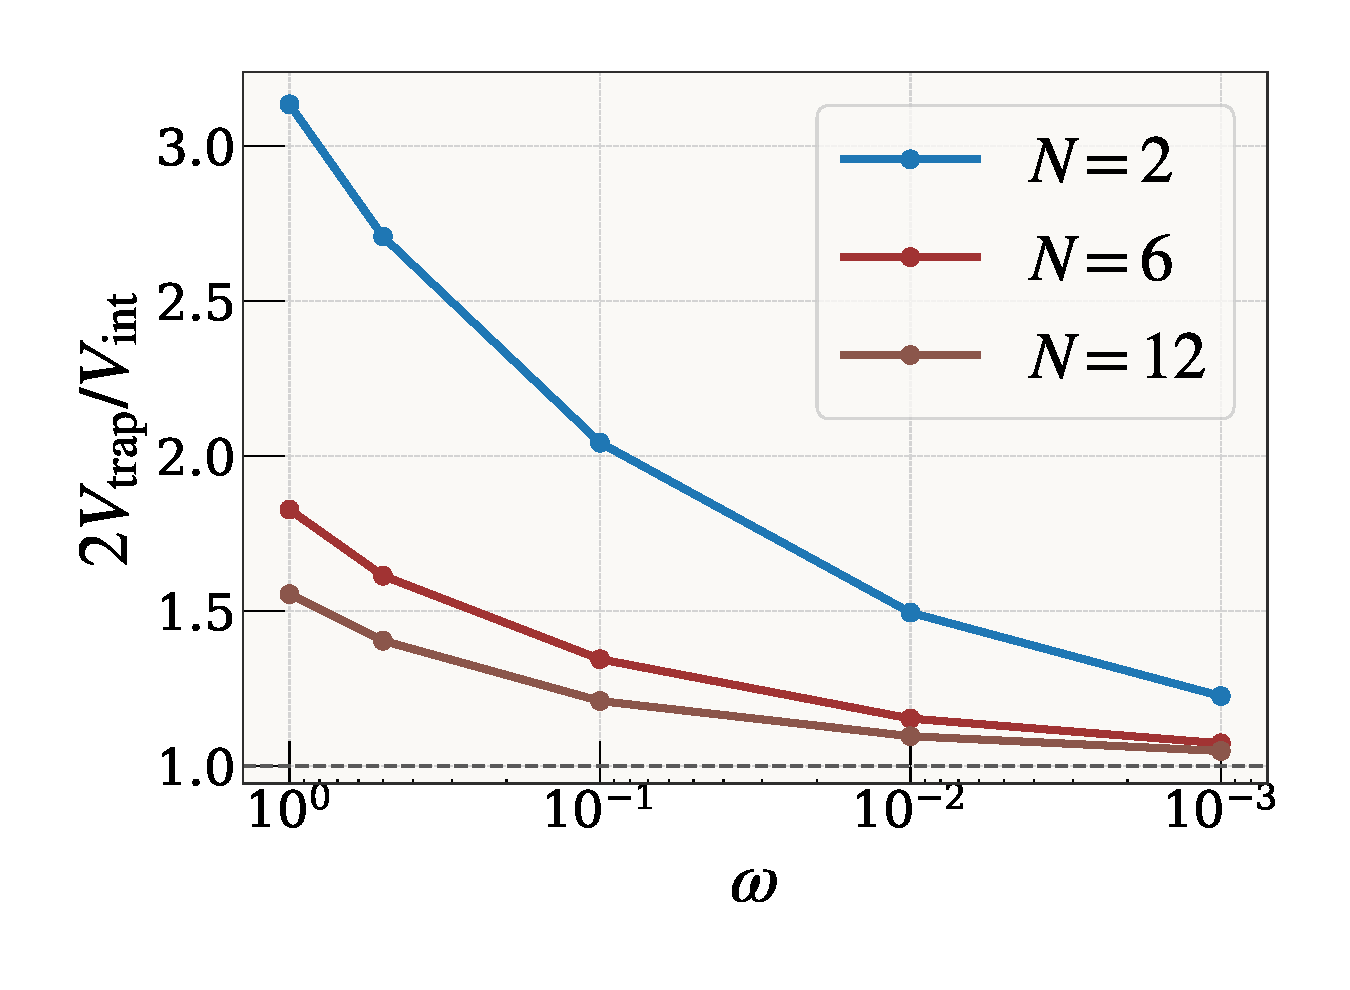
\includegraphics[width=\linewidth]{ratio_2Vtrap_over_Vint_desc_allN}
    \caption[]{$2V_{\rm trap}/V_{\rm int}$ vs.\ $\omega$ for $N{=}2,6,12$.
    The horizontal line marks the classical virial ratio $2V_{\rm trap}=V_{\rm int}$.}
  \end{subfigure}

  \caption[Energy-based Wigner diagnostics against trap frequency]{Energy-based Wigner diagnostics as functions of trap frequency.
  As $\omega$ decreases the dots become interaction dominated
  ($T/V_{\rm int}\!\ll1$) and the trap--interaction partition approaches the
  classical virial form, most clearly for $N{=}12$.}
  \label{fig:wigner_ratios}
\end{figure*}

The energy partition carries two messages, and only two.

\emph{Interactions take over.} The interaction-to-kinetic ratio
$\Gamma=\langle V_{\rm int}\rangle/\langle T\rangle$ rises across
$\omega\in[1,10^{-3}]$ from $0.9$ to $8.6$ at $N{=}2$, from $2.4$ to $24.5$ at $N{=}6$ and
from $3.6$ to $41.1$ at $N{=}12$ (Fig.~\ref{fig:wigner_ratios}a). The dot stops being a
kinetic-energy-dominated droplet and becomes a Coulomb-dominated one.

\emph{Classical force balance emerges.} At $\omega=10^{-3}$ the trap--interaction partition
$2\langle V_{\rm trap}\rangle/\langle V_{\rm int}\rangle$ reaches $1.23$, $1.07$ and $1.05$
at $N=2,6,12$, so the twelve-electron dot satisfies the classical condition
$V_{\rm int}\approx2V_{\rm trap}$ to within $5\%$ (Fig.~\ref{fig:wigner_ratios}b). The
approach is monotone and improves with $N$, as it should: the classical limit is reached
faster when there are more particles to arrange.

Both are consistent with real-space expansion. The rms radius extracted from
$V_{\rm trap}=\tfrac12\omega^2\sum_i\langle r_i^2\rangle$ grows from $1.1$--$2.0\,a_B^\ast$
at $\omega=1$ to $70$--$170\,a_B^\ast$ at $\omega=10^{-3}$, faster than the non-interacting
$\omega^{-1/2}$ law, which is interaction-driven swelling. The fitted exponents for the
individual energy components and for the radius, which support these statements without
adding to them, are collected in Appendix~\ref{app:energy-exponents}.

% ──────────────────────────────────────────────────────────────────────
\subsection{Radial localisation and pair correlations}
\label{sec:wigner-radial}

Over the weakest three confinements, the typical one-body radius follows
$r_{\rm mode}\!\sim\!\omega^{\alpha}$ with $\alpha\simeq-0.626$ at $N{=}2$---close to
the classical two-body value $-2/3$, which nothing in the ansatz knows about. At $N{=}2$ the
width-to-scale ratio $\gamma=\sigma_r/r_{\rm mode}$ falls as well, from $0.49$ to $0.29$, so
the pair stiffens rather than merely dilating. At $N{=}6$ the same global ratio barely moves
(Table~\ref{tab:radial-compact}), and radial stiffening there has to be read from quantities
that resolve the shell, not from this one.

\begin{table}[H]
\centering
\caption[Radial localisation across the confinement range]{Radial localisation across the confinement range. $r_{\rm mode}$ is the mode of
the single-particle radial density in Bohr; $\gamma=\sigma_r/r_{\rm mode}$ is the
width-to-scale ratio. Full diagnostics---mean, width, FWHM, quantiles, ring-angle spread
and pair Lindemann ratio---are in Appendix~\ref{app:structural-tables}. The $N{=}6$ values
at $\omega\le0.01$ come from an earlier run than the shell analysis and
Fig.~\ref{fig:6N_radial_densities} (Appendix~\ref{app:reproducibility}).}
\label{tab:radial-compact}
\begin{tabular}{lcccc}
\toprule
 & \multicolumn{2}{c}{$N{=}2$} & \multicolumn{2}{c}{$N{=}6$} \\
\cmidrule(lr){2-3}\cmidrule(lr){4-5}
$\omega$ & $r_{\rm mode}$ & $\gamma$ & $r_{\rm mode}$ & $\gamma$ \\
\midrule
1.00  & $1.44$  & $0.491$ & $2.09$   & $0.442$ \\
0.50  & $2.30$  & $0.437$ & $3.07$   & $0.445$ \\
0.10  & $3.60$  & $0.480$ & $8.17$   & $0.429$ \\
0.01  & $14.19$ & $0.396$ & $33.15$  & $0.420$ \\
0.001 & $64.29$ & $0.287$ & $113.55$ & $0.421$ \\
\bottomrule
\end{tabular}
\end{table}

The exponent is not the sharpest form of this check. Because $r_{\rm mode}$ is the mode of
the \emph{single-particle} radial density, it mixes the central electron of a $(1,5)$
topology with the ring and is not the ring radius. The shell-resolved outer radius is, and
comparing it with the classical Wigner ring $1.334\,\omega^{-2/3}$ tests a prefactor as
well as a power. That ratio falls monotonically---$1.247$, $1.188$, $1.098$, $1.032$,
$1.017$ from $\omega=1$ to $10^{-3}$---so at the weakest trap the quantum ring sits $1.7\%$
outside the classical one, and the fitted exponent on that quantity is $-0.637$ over the
full grid and $-0.650$ over the weakest three confinements
(Appendix~\ref{app:structural-tables:radius}). Nothing in the ansatz, the objective or the
sampler knows the number $1.334$.

The two sizes stiffen differently, and the difference is physical. At $\omega=10^{-3}$
the $N{=}2$ pair sits at separation $r_{12}\!\approx\!122$ with Lindemann ratio
$\gamma_{r_{12}}\!\approx\!0.20$ and a relative angle sharply peaked at $\pi$: a dilute,
anti-aligned dimer. At $N{=}6$ the global $\gamma$ plateaus near $0.42$, and the evidence
for stiffening comes from the shell-resolved and pair quantities instead: the outer ring's
own relative radial width falls from $0.32$ at $\omega=1$ to $0.15$ at $10^{-3}$
(Table~\ref{tab:shell-summary}), and the ring's angular fluctuations and pair Lindemann
ratio fall monotonically. A single-particle width is the weakest of the radial diagnostics:
it mixes the central electron with the ring, and it is the one quantity here that does not
resolve the shell structure it is being asked about.

\begin{figure}[htp]
  \centering
  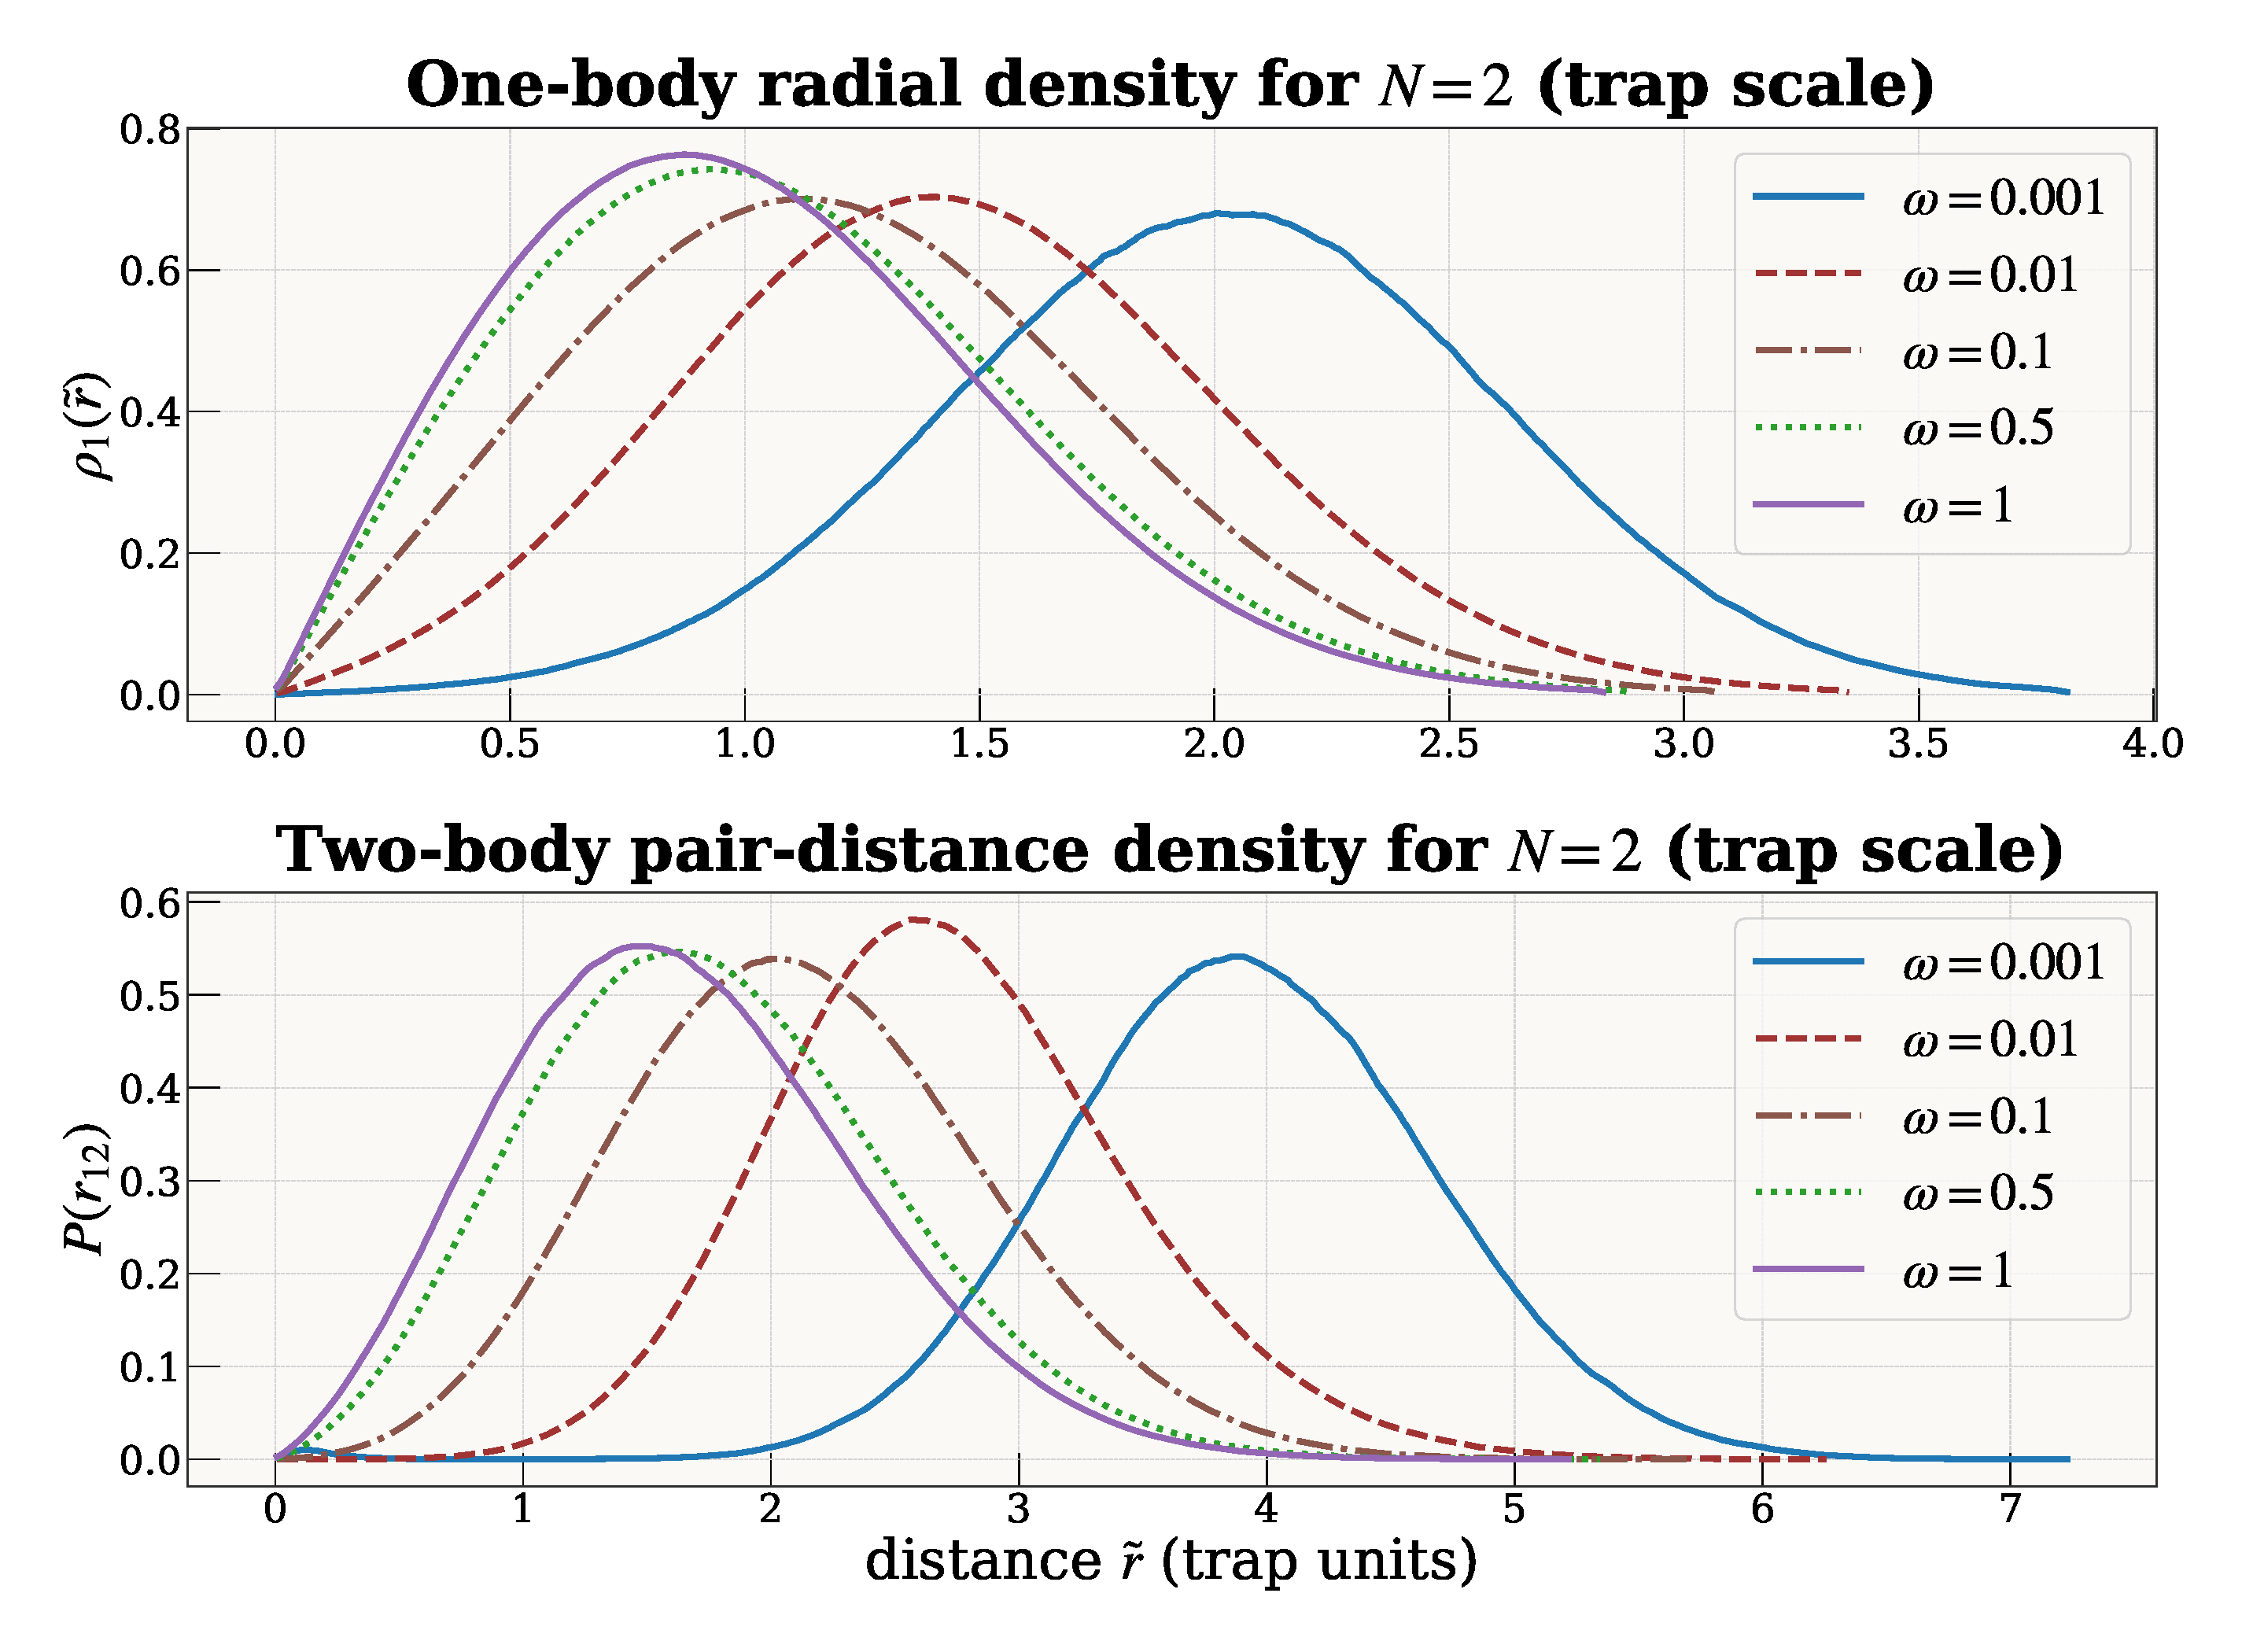
\includegraphics[width=0.9\textwidth]{N2_all_densities}
  \caption[Two-electron radial and pair-distance densities]{One-body radial density
  $\rho_1(\tilde r)$ (top) and pair-distance density $P(r_{12})$ (bottom) for $N{=}2$ across
  $\omega$, in trap units $\tilde r=\sqrt\omega\,r$.}
  \label{fig:2N_radial_densities}
\end{figure}

\begin{figure}[htp]
  \centering
  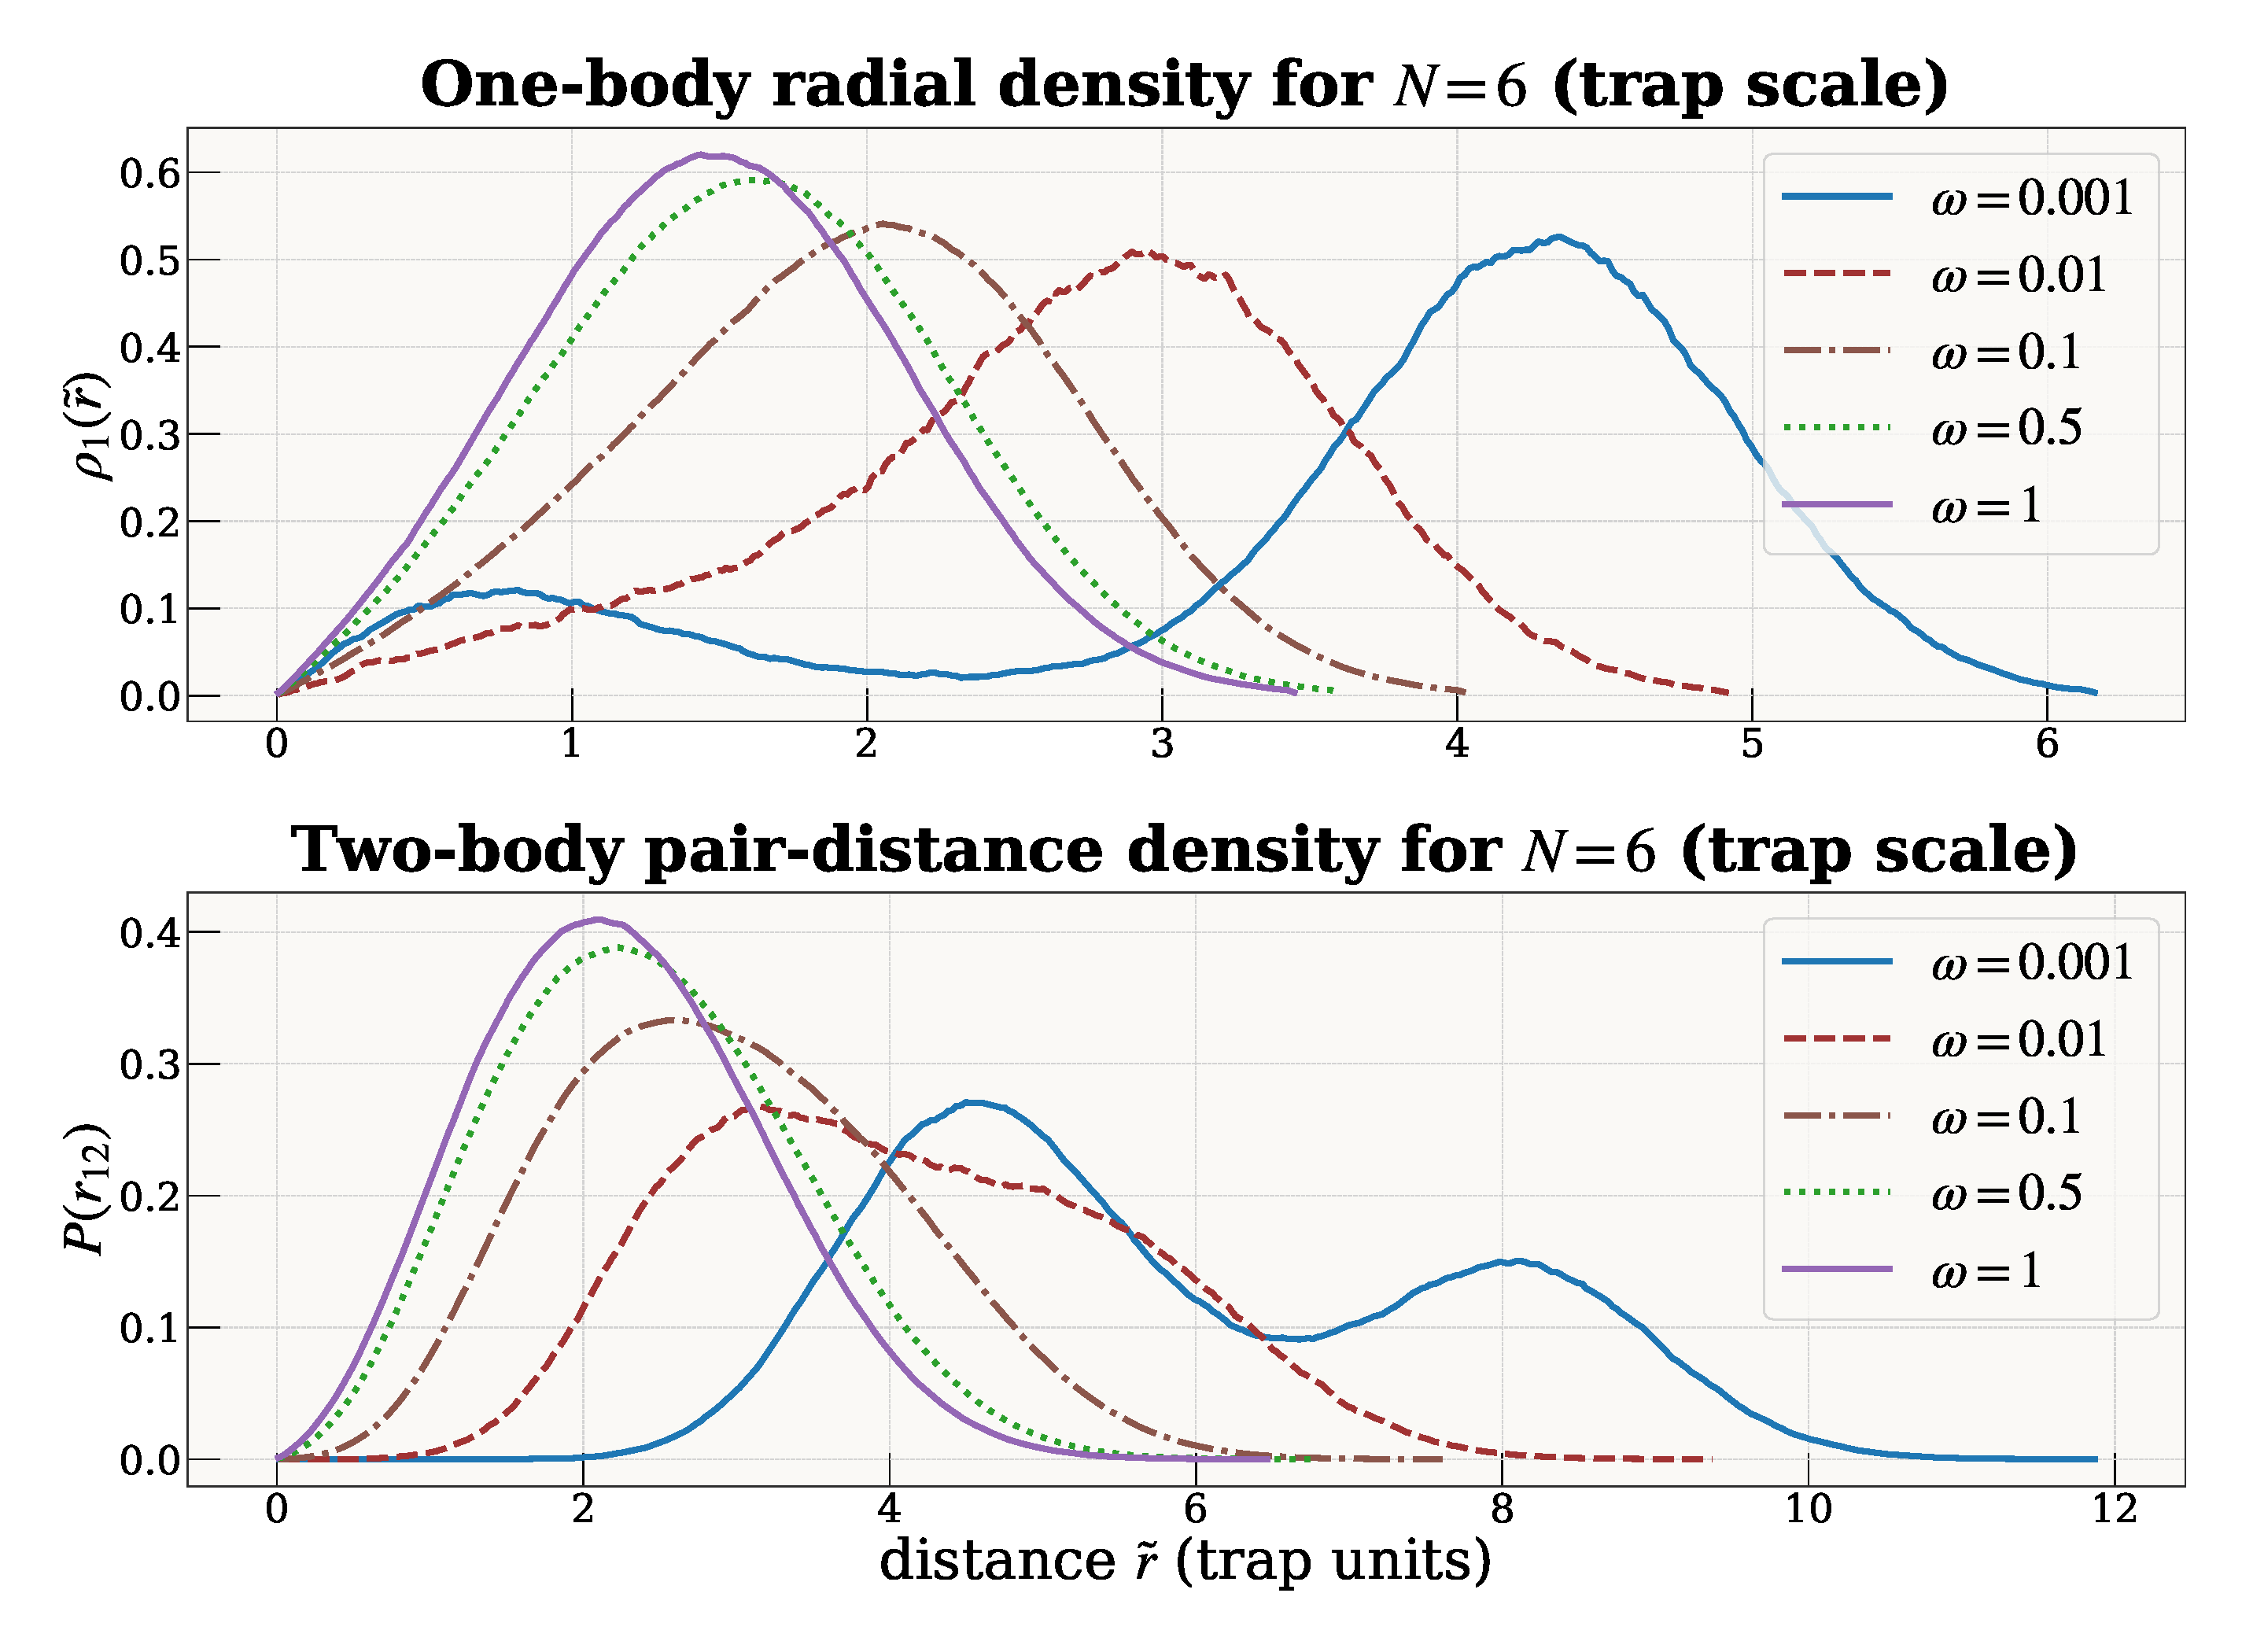
\includegraphics[width=0.9\textwidth]{N6_all_densities}
  \caption[Six-electron radial and pair-distance densities]{As
  Fig.~\ref{fig:2N_radial_densities}, for $N{=}6$. At $\omega=10^{-3}$ the one-body density
  separates into the central electron and the ring, and the pair distribution splits into
  centre--ring and nearest-neighbour distances (first peak) and cross-ring distances
  (second).}
  \label{fig:6N_radial_densities}
\end{figure}

% ──────────────────────────────────────────────────────────────────────
\subsection[Shell topology and angular order]{Shell topology, angular order, and the rotating Wigner molecule}
\label{sec:wigner-angular}

The densities plotted above look like smooth rings, yet the electrons are localised. Both
are true, and the reason is symmetry. Because the Hamiltonian is rotationally invariant, so is its ground state, and any lab-frame
average necessarily smears an angularly ordered configuration into a featureless
ring. The order is real; it simply lives in relative coordinates, and looking for it
in the lab frame is looking in the one place it is guaranteed not to be. Everything
below follows from taking that seriously.

Concretely, a Wigner molecule's internal angular order can only be observed after
registering frames to a co-rotating reference.
For a shell $s$ with $n_s$ particles we compute a rotation-registered
bond-orientational parameter $|\Phi_{n_s}|$ and a corresponding
Lindemann-type ratio quantifying angular stiffness.  Lab-frame densities
remain ring-like (the ``rotating Wigner molecule'' scenario), while the
co-rotating frame reveals crystal-like polygon
order~\cite{Egger_1999,manninen2007metalclustersquantumdots}.

\paragraph{$N{=}6$: single ring with sector mixing.}
At $\omega=0.01$ the system fluctuates between a $(1,5)$ sector (fraction
$\approx 0.69$) and a $(0,6)$ single-ring sector (fraction $\approx 0.31$),
with bond order $|\Phi_5|=0.453\pm0.214$ and $|\Phi_6|=0.466\pm0.206$
respectively. Two conventions apply here and below. The quoted $\pm$ is the frame-to-frame
standard deviation of $|\Phi_m|$, not a standard error on its mean, which with $3\times10^4$
frames is smaller by two orders of magnitude. And these are \emph{sector-conditioned} values,
computed on the frames assigned to that sector in an earlier analysis pass than the
modal-topology values of Appendix~\ref{app:structural-tables:shells}; the two estimators are
set side by side in Table~\ref{tab:bondorder-estimators}. Both must be read against the random-angle
null, the exact mean of $|\Phi_n|$ for independent uniform angles
(Eq.~\eqref{eq:phi-null}), which is $0.402$ for $n{=}5$ and $0.366$ for $n{=}6$: the ratios
here are $1.13$ and $1.27$, so the measured bond order at $\omega=0.01$
exceeds the random-angle value by a modest margin rather than sitting on it.
At $\omega=10^{-3}$ the ring stiffens further:
$(1,5)$ fraction $\approx 0.80$, $(0,6)\approx 0.20$, with
$|\Phi_5|=0.597\pm0.224$ (Lind$\,\approx\!0.225$) and
$|\Phi_6|=0.663\pm0.183$ (Lind$\,\approx\!0.205$)---now far above the random-angle null,
by factors of $1.49$ and $1.81$. This is the confinement at which $n$-fold angular order
becomes \emph{large} rather than merely resolvable
(Appendix~\ref{app:structural-tables:shells}). The distinction matters because with
$10^4$--$10^6$ frames a $2\%$ excess over the null is already resolved at tens of standard
errors; detectability is therefore not what separates the regimes, magnitude is.
Classically $(1,5)$ is the ground-state topology and $(0,6)$ a proximate
competitor; the observed quantum mixture mirrors this
hierarchy~\cite{schweigert1994spectralpropertieschargedparticles,Kong_2002}.
In both weak-trap cases the global $g(r)$ is reproduced to numerical
precision by the appropriate inner--inner / inner--outer / outer--outer (II/IO/OO) mixtures.

\paragraph{$N{=}12$: two shells and commensurability.}
At $\omega=0.01$ two-shell formation is already frequent (fraction $0.761$ at
radial-gap threshold $\tau{=}3.0$), distributed across sectors
$(1,11)=32.6\%$, $(2,10)=25.7\%$, $(3,9)=13.7\%$.
At $\omega=10^{-3}$ shelling becomes ubiquitous
($f_{\rm 2shell}\!\approx\!0.99$--$0.92$ for $\tau=2.0$--$3.0$) and the
\emph{commensurate} $(3,9)$ split emerges as modal ($43.3\%$ of quality-cut
frames), with strong bond order on both rings:
$|\Phi_3|=0.687\pm0.229$ (Lind$_{\rm in}=0.223$),
$|\Phi_9|=0.526\pm0.194$ (Lind$_{\rm out}=0.224$).
Whether the shell picture actually explains the pair structure needs a test that could
fail, and the obvious one cannot. Recombining the inner--inner, inner--outer and
outer--outer histograms with the combinatorial weights of the ideal $(3,9)$ topology
reproduces the global $g(r)$ essentially exactly---but the sector histograms and the total
are accumulated from the same frames, so that recombination is close to exact by
construction. It establishes that the sector bookkeeping is self-consistent, nothing more,
and it is recorded in Appendix~\ref{app:structural-tables:mixfit} for that reason.

The test that can fail is generative and held out (Table~\ref{tab:shell-model-fit-main}).
Shell radii and widths are fitted on half the frames; each shell is modelled as a regular
$n_s$-gon carrying a per-frame global rotation and a fitted angular jitter; and the model is
scored on the other half. It reproduces the pair distribution to cosine similarity
$0.987$--$0.999$ across the whole grid, against $0.936$--$0.996$ for an angle-randomised
null built from the same fitted radial distributions. The difference between them,
$\Delta\cos$, is what \emph{angular} order buys over shell radii alone, and it grows
monotonically as the trap weakens at every particle number---at $N{=}12$ from $0.006$ at $\omega=1$ to $0.026$ at $\omega=10^{-3}$, at $N{=}6$ from
$0.012$ to $0.058$, at $N{=}20$ from $0.003$ to $0.010$. Shell radii alone account for most
of the pair structure at strong confinement; angular structure accounts for a growing
remainder as the molecule forms. How firmly is a separate question, because the smallest
values are a few thousandths, and it was tested directly
(Appendix~\ref{app:structural-tables:mixfit}). Every $\Delta\cos$ carries a block-bootstrap
interval that excludes zero---at $N{=}20$, $\omega=1$ it is $[0.0027,0.0030]$---and the
growth with $1/\omega$ is resolved at every particle number. It survives changes of histogram
binning and of the train/test split essentially unchanged. What does move it is the
angular-jitter model, by up to a third, and the shell threshold where that changes the
partition; the size of $\Delta\cos$ is model-dependent, its sign and its trend are not.

That growth has a different shape from the bond order. $\Delta\cos$ rises by a factor of
$1.1$--$2.1$ per decade at every particle number, monotonically and without a threshold,
whereas the bond order stays flat at its null and then jumps. The two are not in conflict:
$\Delta\cos$ responds to \emph{any} angular correlation that improves the pair-distance
density, while $|\Phi_n|$ responds specifically to $n$-fold order on a registered ring. Weak
angular correlations build gradually from strong confinement onward, and crystalline $n$-fold
order emerges from them only in the final decade---three stages, not a single threshold, with
the middle one measured by a quantity whose sign and trend are robust but whose size depends
on the shell model.

\begin{table}[htbp]
\centering
\caption[Held-out shell-model fit against an angle-randomised null]{The structural test
that can fail. Shell radii and widths are fitted on half the frames; each detected shell is
then modelled as a regular $n_s$-gon carrying a per-frame global rotation and a fitted
angular jitter; and the resulting pair-distance density is scored on the \emph{held-out}
half. $\cos_{\rm poly}$ is the polygon model's agreement with the empirical density and
$\cos_{\rm uni}$ that of an angle-randomised null with the same fitted radial
distributions, so $\Delta\cos$ isolates what polygonal order contributes over shell radii
alone. The interval is a $95\%$ block bootstrap over frames that refits the model and draws
a fresh model sample in every replicate; the tabulated point uses the original single model
sample, whose Monte Carlo noise is part of what the interval measures, so a point can sit
near an edge. Sensitivity to binning, split, shell threshold and jitter model is in
Appendix~\ref{app:structural-tables:mixfit}, with the full table and residuals.}
\label{tab:shell-model-fit-main}
\small
\setlength{\tabcolsep}{6pt}
\begin{tabular}{ccl cccc}
\toprule
$N$ & $\omega$ & occ. & $\cos_{\rm poly}$ & $\cos_{\rm uni}$ & $\Delta\cos$ & $95\%$ interval \\
\midrule
6 & $1.0$ & $1,5$ & $0.9988$ & $0.9866$ & $\mathbf{0.0122}$ & $[0.0122,\,0.0136]$ \\
6 & $0.5$ & $1,5$ & $0.9986$ & $0.9836$ & $\mathbf{0.0150}$ & $[0.0147,\,0.0160]$ \\
6 & $0.1$ & $1,5$ & $0.9974$ & $0.9741$ & $\mathbf{0.0234}$ & $[0.0219,\,0.0236]$ \\
6 & $0.01$ & $1,5$ & $0.9922$ & $0.9536$ & $\mathbf{0.0386}$ & $[0.0371,\,0.0395]$ \\
6 & $0.001$ & $1,5$ & $0.9942$ & $0.9358$ & $\mathbf{0.0585}$ & $[0.0556,\,0.0592]$ \\
\midrule
12 & $1.0$ & $1,11$ & $0.9993$ & $0.9937$ & $\mathbf{0.0056}$ & $[0.0054,\,0.0059]$ \\
12 & $0.5$ & $1,11$ & $0.9990$ & $0.9927$ & $\mathbf{0.0063}$ & $[0.0060,\,0.0066]$ \\
12 & $0.1$ & $1,11$ & $0.9980$ & $0.9896$ & $\mathbf{0.0085}$ & $[0.0083,\,0.0088]$ \\
12 & $0.01$ & $1,11$ & $0.9929$ & $0.9805$ & $\mathbf{0.0124}$ & $[0.0124,\,0.0132]$ \\
12 & $0.001$ & $3,9$ & $0.9868$ & $0.9604$ & $\mathbf{0.0264}$ & $[0.0258,\,0.0271]$ \\
\midrule
20 & $1.0$ & $1,19$ & $0.9992$ & $0.9964$ & $\mathbf{0.0028}$ & $[0.0027,\,0.0030]$ \\
20 & $0.5$ & $1,19$ & $0.9990$ & $0.9958$ & $\mathbf{0.0032}$ & $[0.0030,\,0.0033]$ \\
20 & $0.1$ & $1,19$ & $0.9982$ & $0.9942$ & $\mathbf{0.0040}$ & $[0.0038,\,0.0040]$ \\
20 & $0.01$ & $1,19$ & $0.9947$ & $0.9900$ & $\mathbf{0.0047}$ & $[0.0046,\,0.0049]$ \\
20 & $0.001$ & $1,7,12$ & $0.9915$ & $0.9820$ & $\mathbf{0.0095}$ & $[0.0091,\,0.0095]$ \\
\bottomrule
\end{tabular}
\end{table}



\begin{figure}[htp]
  \centering
  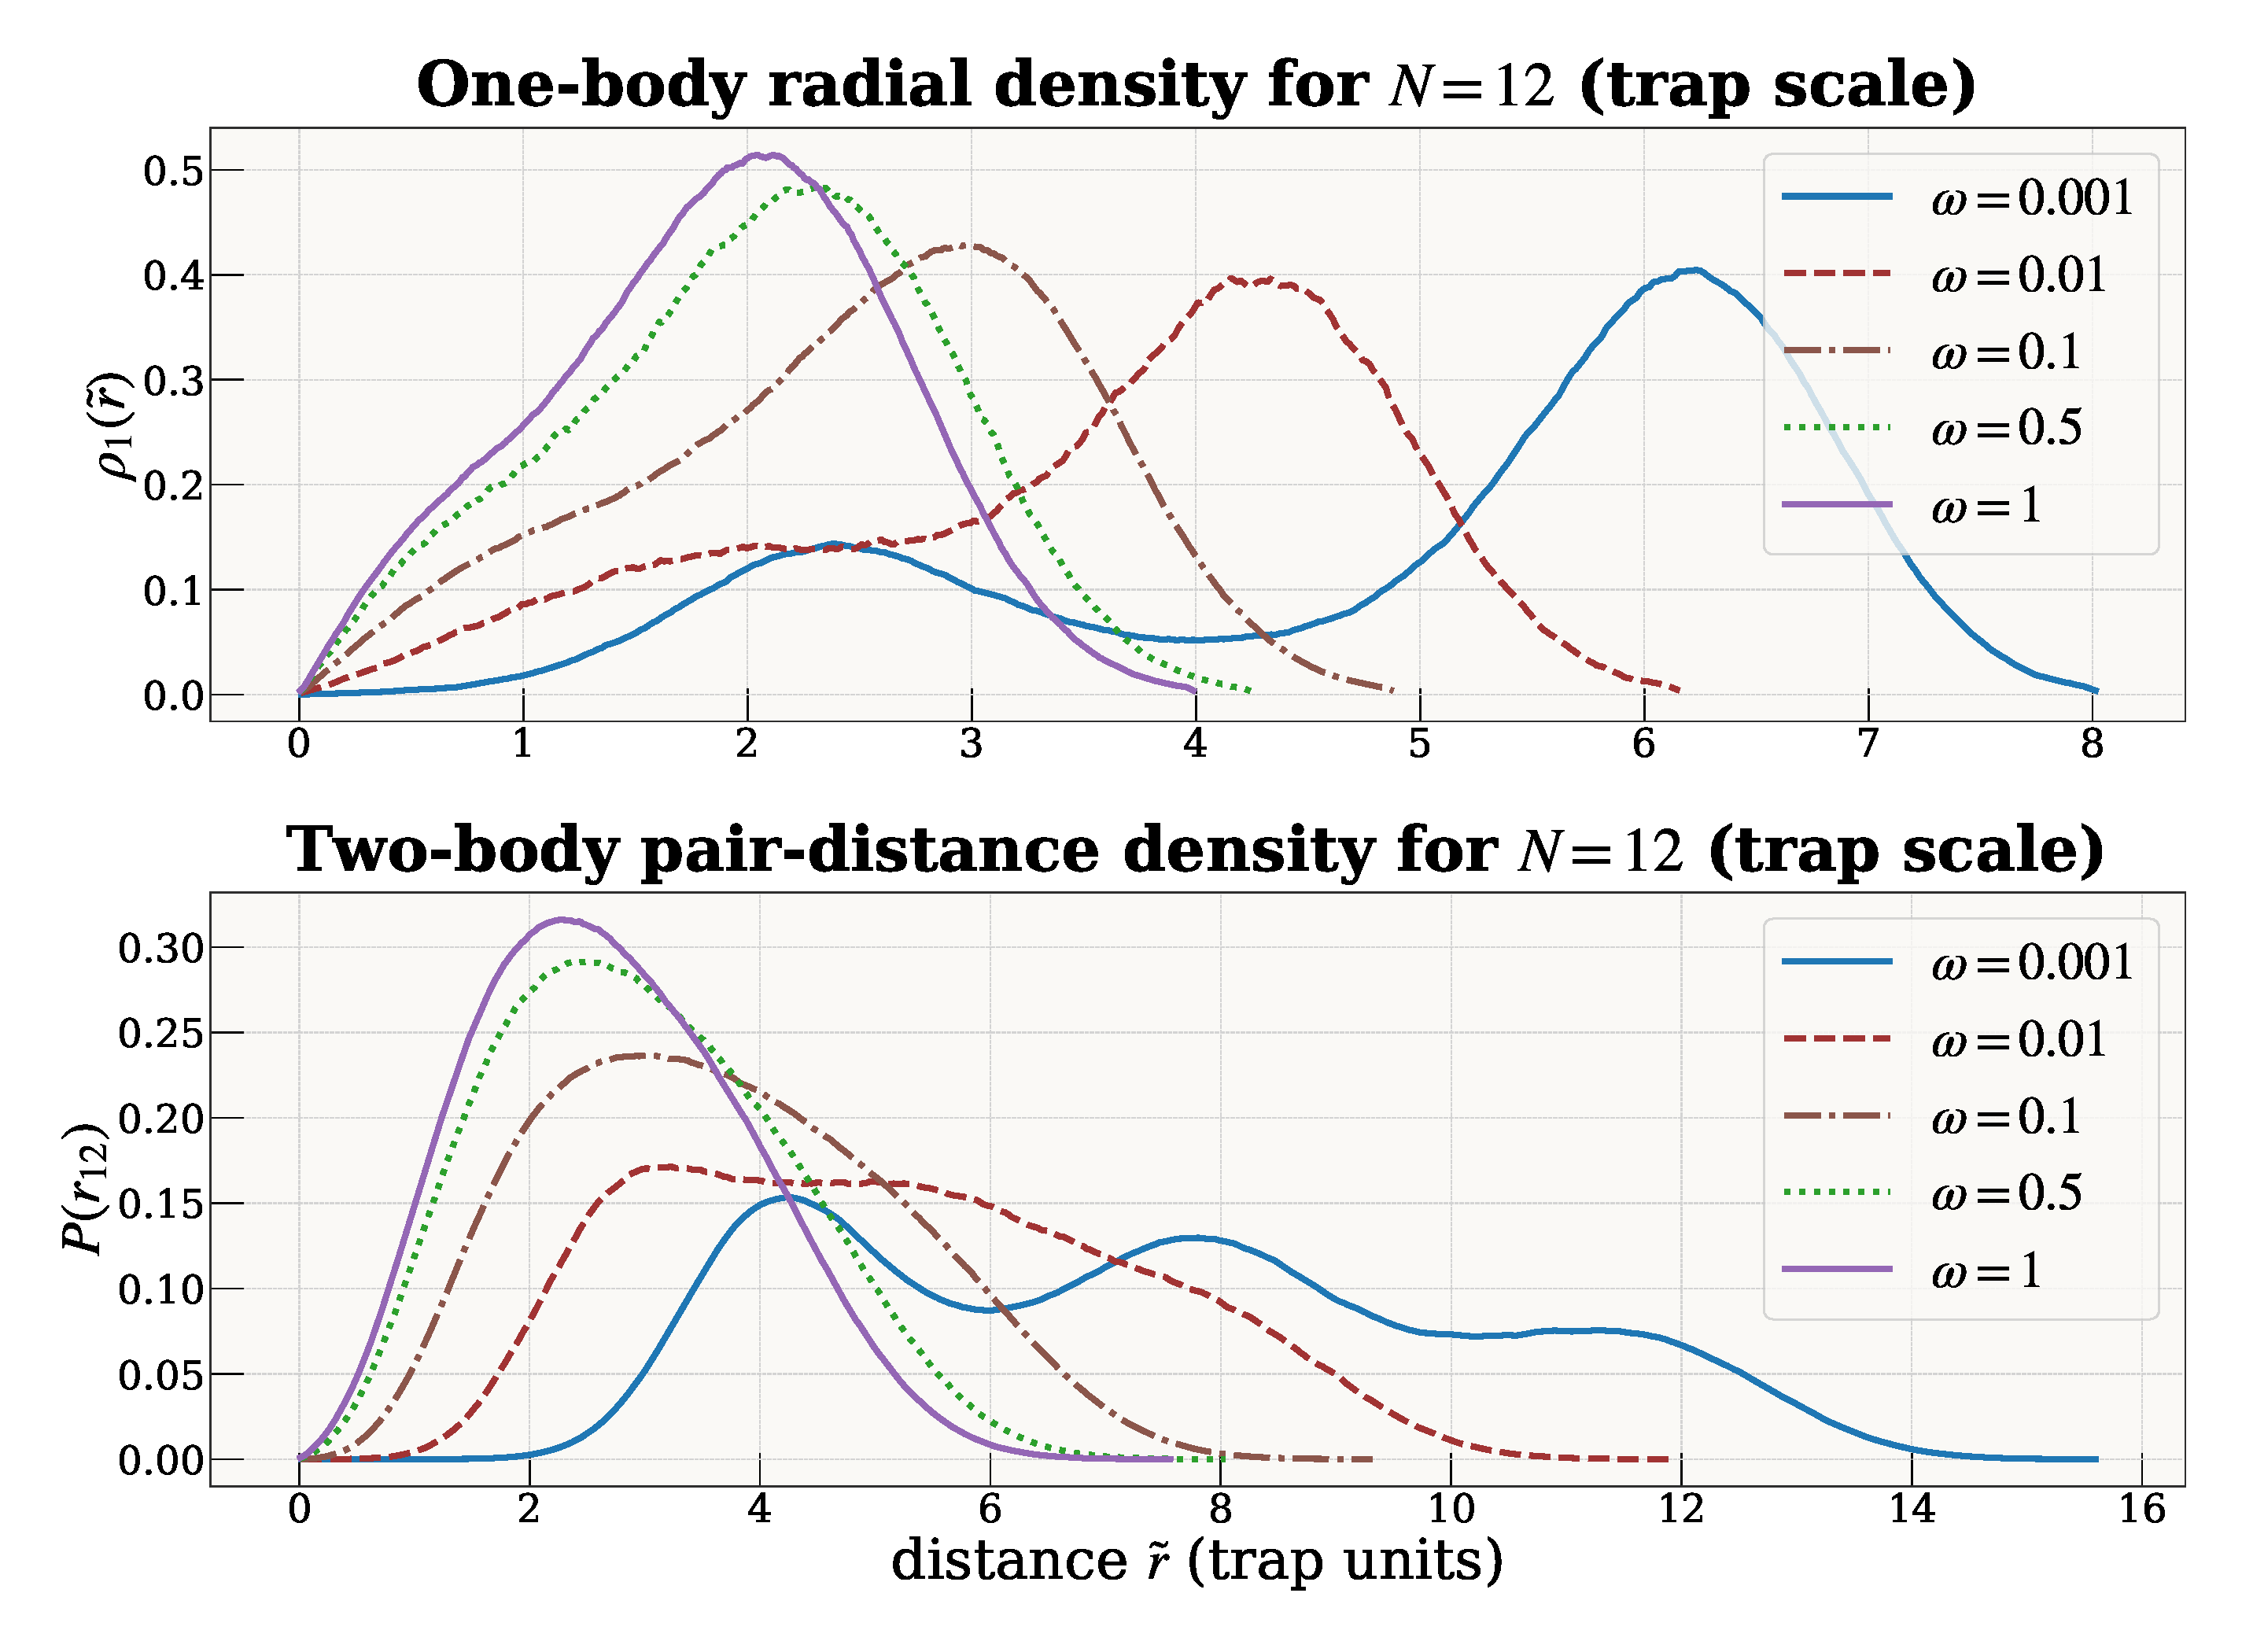
\includegraphics[width=0.9\textwidth]{N12_all_densities}
  \caption[Twelve-electron radial and pair-distance densities]{As
  Fig.~\ref{fig:2N_radial_densities}, for $N{=}12$.}
  \label{fig:12N_radial_densities}
\end{figure}

\paragraph{$N{=}20$: three-shell molecule and a rapid radial reorganisation.}
At $\omega=10^{-3}$ the dominant shell topology is $(1,7,12)$---a clear
three-shell Wigner molecule with widely separated rings at radii
$r_0\approx38$, $r_1\approx132$, $r_2\approx247$
(gaps $\approx94$ and $\approx115$).
The lab-frame pinning metric remains small ($C_{\mathrm{global}}\approx0.06$), as expected
for a freely rotating molecule. That number also answers a question the ansatz raises. Its
displacement head is not rotation-equivariant by construction (\S\ref{sec:bf-init}), so a
trained state could in principle carry an orientation fixed to the lab frame and read as
angular order; such a state would show a large $C_{\mathrm{global}}$, and this one does not.
The order the per-shell moduli measure is internal to the molecule. The cross-shell quantity $\tilde C_{\mathrm{global}}$ is
omitted: it depends on a registration convention whose original analysis code was not
retained (\S\ref{subsec:orient}). The per-shell moduli and angular-spacing diagnostics below
are rotation-invariant and carry no such dependence.
Lindemann disorder on the two occupied outer shells is low:
$L_{7,\mathrm{reg}}\approx0.35$ and
$L_{12,\mathrm{reg}}\approx0.27$.

Already at $\omega=10^{-2}$ the radial gap detector returns a $(1,19)$ partition rather than
a three-shell one: the shell radii contract by an order of magnitude ($r_0\approx10$,
$r_1\approx45$), the outer-shell angular disorder rises to $\approx0.57$. The wording
matters here. At $\omega=10^{-3}$ the $(1,7,12)$ label describes a
Wigner \emph{topology}, because it is accompanied by separated shells, registered angular
order and low Lindemann disorder. At $\omega=10^{-2}$ and above, with angular order at its
random-angle null and disorder high, $(1,19)$ is what the \emph{radial classifier returns}
on a state that is not angularly ordered at all---a decomposition of the radial density, not
a crystalline shell structure. We use the occupancy notation in both cases because the
detector does, but only the weakest-trap case earns the word topology.
At $\omega=1$ the classifier returns the same $(1,19)$ partition, with compact radii
($r_0\approx0.55$, $r_1\approx2.3$) and high angular disorder
($L_{\rm out}\approx0.69$).
What the data show, then, is a rapid radial reorganisation somewhere between
$\omega=10^{-3}$ and $10^{-2}$, not a collapse of one crystalline topology into another: the
state at $10^{-2}$ has no demonstrated angular order to lose. How rapid, and where in that
decade it happens, the grid cannot say. It samples one point per decade, and the radial
classifier reports a partition at each point rather than tracking a structure between them.

\subsection{The crossover across diagnostics}
\label{sec:wigner-synthesis}

Six diagnostics, applied at four particle numbers and five confinements, agree. As $\omega$
falls from $1$ to $10^{-3}$ the densities expand and develop rings, and the shell topology
resolves into the discrete finite-$N$ patterns that classical Coulomb clusters
predict---$(1,5)$ at $N{=}6$, $(3,9)$ at $N{=}12$, $(1,7,12)$ at
$N{=}20$~\cite{schweigert1994spectralpropertieschargedparticles,Kong_2002}. The shells
separate and stiffen. The Lindemann disorder falls monotonically throughout, while
rotation-registered bond order stays within $1\%$ of its random-angle null down to
$\omega=0.1$ and reaches $1.16$--$1.63$ times it only at $\omega=10^{-3}$
(Appendix~\ref{app:structural-tables:shells}). Radial stiffening precedes $n$-fold angular ordering instead of accompanying it. Lab-frame order stays near zero throughout, as
expected for a freely rotating molecule.
The energy partitioning approaches the classical virial form, with $\Gamma$ reaching
${\sim}40$ for $N{=}12$ at the weakest trap. None of these was built into the ansatz. The commensurate $(3,9)$ sector at $N{=}12$ carries real weight in
$(1,11)$ and $(2,10)$ besides, which is the quantum rotational mixing the rotating-Wigner-molecule
picture
predicts~\cite{manninen2007metalclustersquantumdots,Filinov_2001}. At $N{=}20$ the
three-shell structure at $\omega=10^{-3}$ gives way, by $\omega=10^{-2}$, to a radial
partition of a state without angular order; the grid is too coarse to place that
reorganisation more finely than within the decade. The $(1,7,12)$ configuration itself is not new. It is the known classical shelling, reported in quantum calculations of comparable dots, and no novelty is claimed for it. What we have not found
reported elsewhere for $N\ge12$ parabolic dots is the combination of \emph{sector-conditioned}
bond-order and Lindemann statistics, read against their random-angle null, with a held-out
polygon reconstruction of $g(r)$ scored against an angle-randomised baseline.

The diagnostics do not carry equal weight, and they do not all support the same claims.
Table~\ref{tab:wigner-evidence} sets out which one carries which statement and how firmly.
The strongest evidence is at the deepest Wigner points; the qualitative staging is better
established than where, within the coarse $\omega$ grid, each stage sets in.

\begin{table}[htbp]
\centering
\caption[Which diagnostic supports which claim]{Which diagnostic supports which claim about
the crossover. ``Firm'' means a large effect in a state-level or shell-resolved quantity;
``weak'' marks evidence that is suggestive but small or carried by a quantity known to
mix structures.}
\label{tab:wigner-evidence}
\small
\renewcommand{\arraystretch}{1.2}
\begin{tabular}{@{}>{\raggedright\arraybackslash}p{0.29\textwidth}
                >{\raggedright\arraybackslash}p{0.42\textwidth}
                >{\raggedright\arraybackslash}p{0.21\textwidth}@{}}
\toprule
Claim & Carried by & Strength \\
\midrule
The cloud expands faster than the non-interacting $\omega^{-1/2}$ &
rms radius from $\langle V_{\rm trap}\rangle$; $r_{\rm mode}$ exponent &
firm, all $N$ \\
Interactions take over &
$\Gamma=\langle V_{\rm int}\rangle/\langle T\rangle$ rises tenfold &
firm, $N\le12$ \\
Classical force balance emerges &
$2\langle V_{\rm trap}\rangle/\langle V_{\rm int}\rangle\to1.23,\,1.07,\,1.05$ &
firm at $N{=}12$ \\
Shells stiffen radially &
shell-resolved widths ($N{=}6$ ring: $0.32\to0.15$) and pair Lindemann ratios; global
$\gamma$ only at $N{=}2$ &
firm; global $\gamma$ weak at $N{=}6$ \\
The ring approaches its classical radius &
outer radius over $1.334\,\omega^{-2/3}$: $1.247\to1.017$ &
firm, $N{=}6$ \\
Discrete Wigner topologies form &
radial classifier with registered order: $(1,5)$, $(3,9)$, $(1,7,12)$ &
firm at $10^{-3}$; above it, radial partitions only \\
Weak angular correlation builds gradually &
held-out polygon model against angle-randomised null, $\Delta\cos$ (block bootstrap) &
firm in sign and trend; size depends on the jitter model \\
$n$-fold angular order appears late &
$|\Phi_n|$ against its exact null, which is also the pipeline's null &
firm at $10^{-3}$; absent above $0.1$ (resolved departures ${\lesssim}1\%$) \\
Where each stage sets in &
one grid point per decade &
not established \\
\bottomrule
\end{tabular}
\end{table}

Two qualifications bound all of it. The states are the lowest we find within a fixed
spin-projection sector, and we have not scanned total spin, so these are not proven
global-spin ground states. And the combinatorial reconstruction of $g(r)$ establishes
decomposability rather than sampling correctness; the held-out polygon fit of
Appendix~\ref{app:structural-tables:mixfit} is the version that could have failed, and
sampling correctness itself rests on the independent restart and chain diagnostics.

The two angular diagnostics stage the crossover slightly differently, and the difference is
informative. Radial localisation (expansion, shell separation, falling shell-resolved width, classical force balance) develops progressively from $\omega=1$ down.
Bond-orientational order is flat at its null through $\omega=0.1$, departs at $\omega=0.01$
clearly only at $N{=}6$, and becomes large at $10^{-3}$ everywhere. The held-out
polygon model, sensitive to any angular correlation rather than to $n$-fold order
specifically, instead grows monotonically throughout, roughly doubling per decade. Read at
face value, weak angular correlations build gradually across the whole range while
\emph{crystalline} $n$-fold order appears only in the last decade: a three-stage picture
rather than a two-stage one. The two-stage separation of radial and $n$-fold angular order
is the firmer statement; the gradual middle stage is resolved in sign and trend, but its size
depends on the shell model used to measure it.

These structural facts then enter the method. The shell radius approaching its classical
$\omega^{-2/3}$ scaling---within $1.7\%$ of the classical prefactor at $\omega=10^{-3}$,
Appendix~\ref{app:structural-tables:radius}---and the angular order sharpening in the last
decade are exactly the quantities a sampler must respect to reach the Wigner regime without a
Markov chain. An origin-centred proposal aims where the wavefunction no longer has any mass;
a proposal built from the measured shell radius and angular order tracks it, and carries
Markov-chain-free training far into the correlated regime
(\S\ref{sec:kernel-q3-frontier}). What the trained model reveals about the physics is what
later lets us train it more cheaply.

That is the state seen from outside. What the network had to hold internally in order to
produce it is a question about the solver, and Chapter~\ref{ch:kernel} takes it up.
